\documentclass[10pt]{beamer}
%\documentclass[10pt,handout]{beamer}

%\usepackage{DSI}
% \usepackage{beamerthemebars}

% \usepackage{beamerthemeboxes}

\useinnertheme[shadow]{rounded}
\usecolortheme{rose}
\usecolortheme{seahorse}
\usecolortheme[rgb={0.0,0.40,0.10}]{structure}

\graphicspath{{../figure/}}

\usepackage[active]{srcltx}

\newcommand{\EM}{\ensuremath}
\newcommand{\ds}[1]{\EM{#1}}
\newcommand{\dsfrac}[2]{\EM{\frac{\ds{#1}}{\ds{#2}}}}

\newcommand{\R}{\EM{\mathbb{R}}}
\newcommand{\C}{\EM{\mathbb{C}}}
\newcommand{\N}{\EM{\mathbb{N}}}
\newcommand{\Z}{\EM{\mathbb{Z}}}
\newcommand{\w}{\EM{\omega}}
\newcommand{\La}[1]{\EM{\mathcal{L}\left[#1\right]}}
\newcommand{\adj}{\EM{\mathrm{adj\,}}}
\newcommand{\vc}{\EM{\mathrm{vec\,}}}
\newcommand{\D}{\EM{\mathcal{D}}}
\newcommand{\eps}{\varepsilon}
\newcommand{\sat}{\mathrm{sat}}
\newcommand{\ellips}{\mathcal{E}}


\newcounter{paragraph}[subsubsection]
\newcommand{\paragraph}{}

\usepackage{times}
\usepackage[T1]{fontenc}
%\usepackage{natbib}
\usepackage{amsmath}
\usepackage{amsthm}
\usepackage{psfrag}
\usepackage{latexsym}
\usepackage{graphicx}


\usepackage{harvard}
\harvardparenthesis{square}
\harvardyearparenthesis{square}


\theoremstyle{plain}
\newtheorem{thm}{Theorem}
\newtheorem{lem}[thm]{Lemma}
\newtheorem{prop}[thm]{Proposition}
\newtheorem*{cor}{Corollary}
\theoremstyle{definition}
\newtheorem{defn}{Definition}
\newtheorem{exmp}{Example}
\theoremstyle{remark}
\newtheorem*{rem}{Remark}

% \mode<presentation>
% {
% % 	\usetheme[secheader]{Boadilla}
%   \usecolortheme[RGB={16,64,128}]{structure}
% }


\title[Less conservative AS criteria]
{Less Conservative Absolute Stability Criteria}

% \subtitle
% {} % (optional)

\author[Materassi] % (optional, use only with lots of authors)
{D.~Materassi\inst{1}}
% - Use the \inst{?} command only if the authors have different
%   affiliation.

% \institute[University of Minnesota]
% {\inst{1}Department of Electrical and Computer Engineering\\ University of Minnesota}

\institute[Universit\`a degli Studi di Firenze]
{\inst{1}Universit\`a degli Studi di Firenze\\
	Dipartimento di Sistemi e Informatica}


\date{\today}
 

\begin{document}

\frame{\titlepage}

\frame{\frametitle{Outline}
	\tableofcontents[pausesections]}

\section{The problem of Absolute Stability}

\frame{\frametitle{Stability for a feedback interconnection}
	\begin{itemize}
		\item In many engineering problems, it is of great importance to study the asymptotic stability of a system described as a feedback interconnection of more subsystems
		\begin{figure}
			\centering
			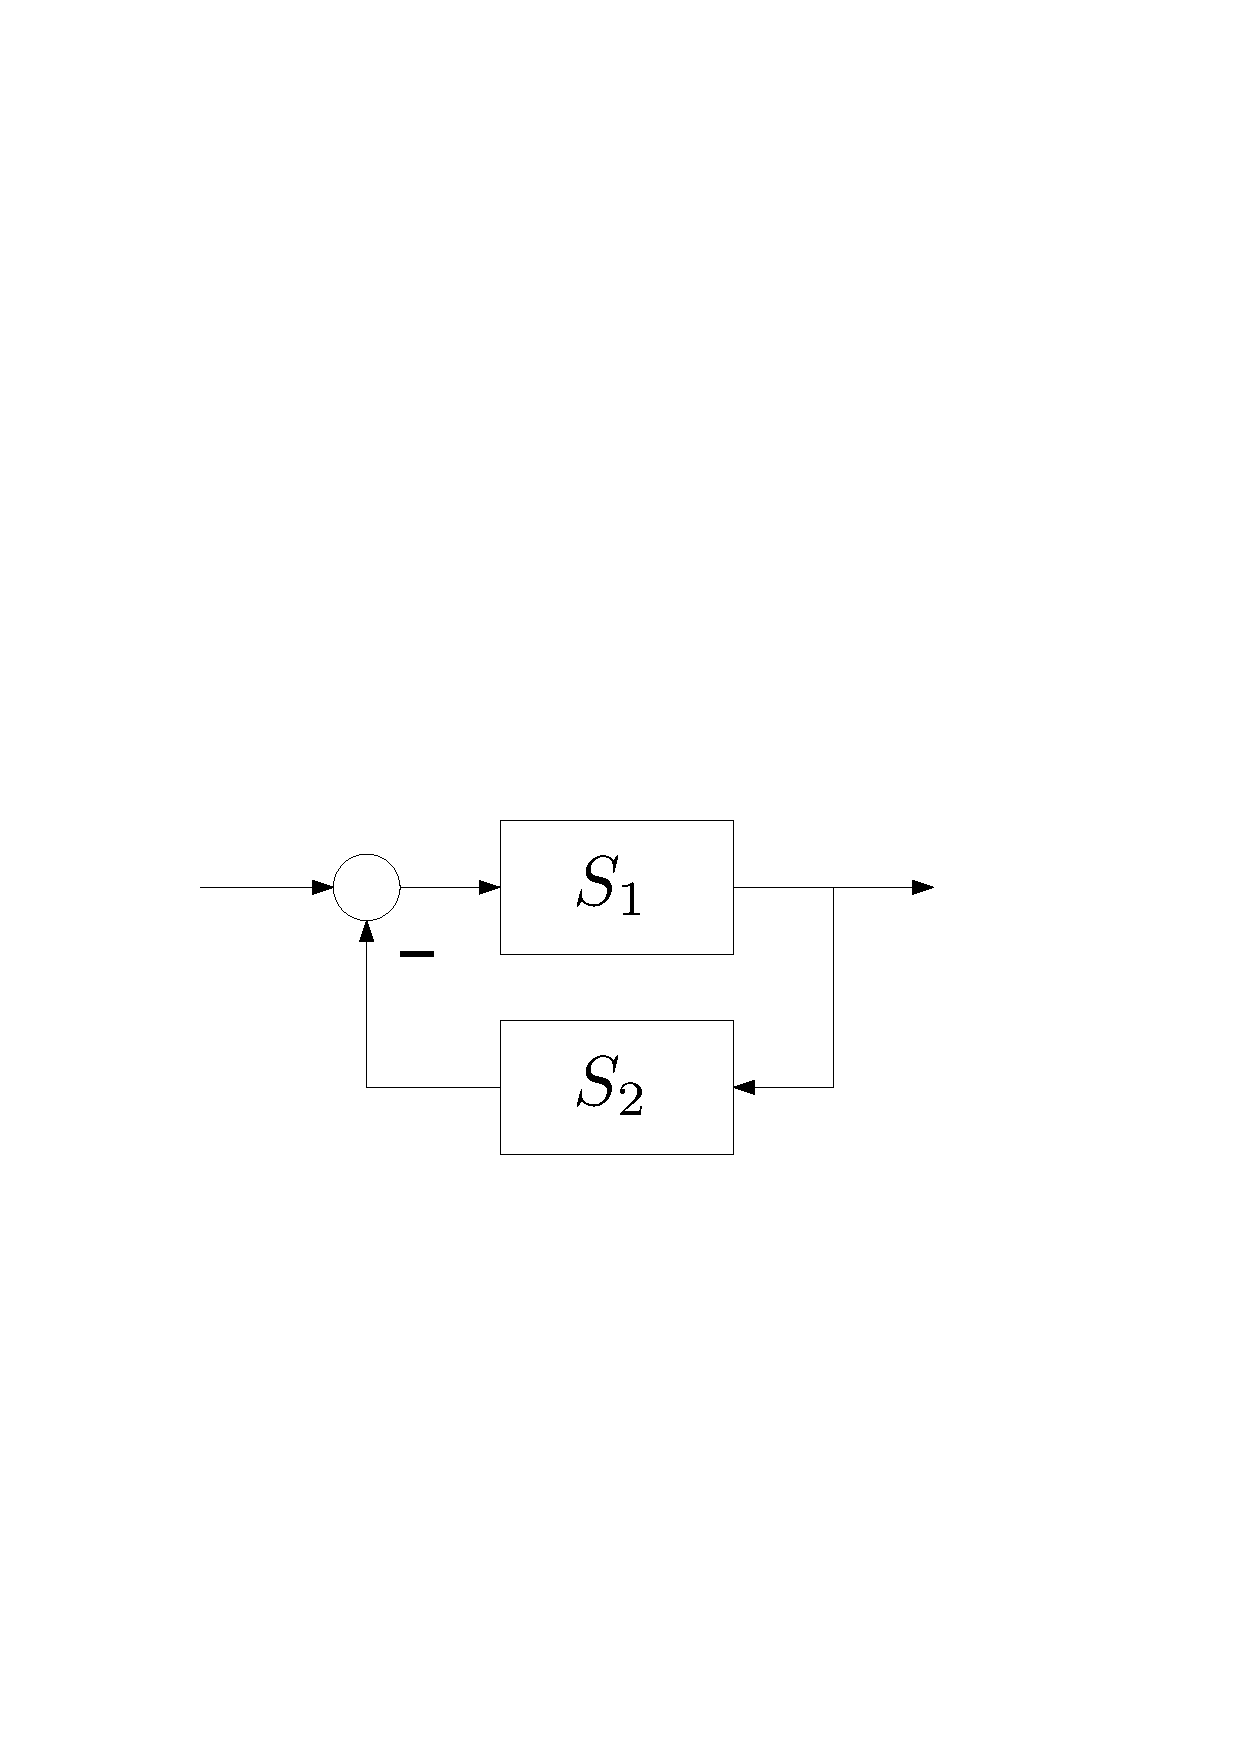
\includegraphics[width=0.6\columnwidth]{feedback}
		\end{figure}
		\item Usually, the theoretical framework where feedback interconnections are studied is the case where all the systems are linear
		\item This approach is useful when we are interested into a ``local description'' of the system (i.e. in the neighborhood of a setpoint condition)
	\end{itemize}
	}

\subsection{Lur'e systems}
\frame{\frametitle{Lur'e systems}
	\begin{itemize}
		\item We resort to nonlinear systems when we are interested into a ``global'' behavior
		\item Linear systems can not show many ``phenomena'' (multiple isolated equilibria, unforced limit cycles, homoclines, heteroclines, deterministic chaos...)
		\item The word ``nonlinear'' is a short form for ``not necessarily linear'', thus being nonlinear is not a actually property
		\item When we are dealing with a nonlinear description of a system, we need to assume at least a structure for it, such as
		\begin{itemize}
			\item Affine
			\item Piecewise linear
			\item Quadratic
			\item ...
		\end{itemize}
	\end{itemize}
}

\frame{\frametitle{Lur'e systems}
	In this talk, we will focus on Lur'e systems
	\smallskip
	\begin{block}{}
		A Lur'e system is given by the feedback interconnection of a Linear Time Invariant (LTI) system $\mathcal{L}$ with a nonlinear memoryless block $\mathcal{N}$
	\end{block}
		\begin{figure}
			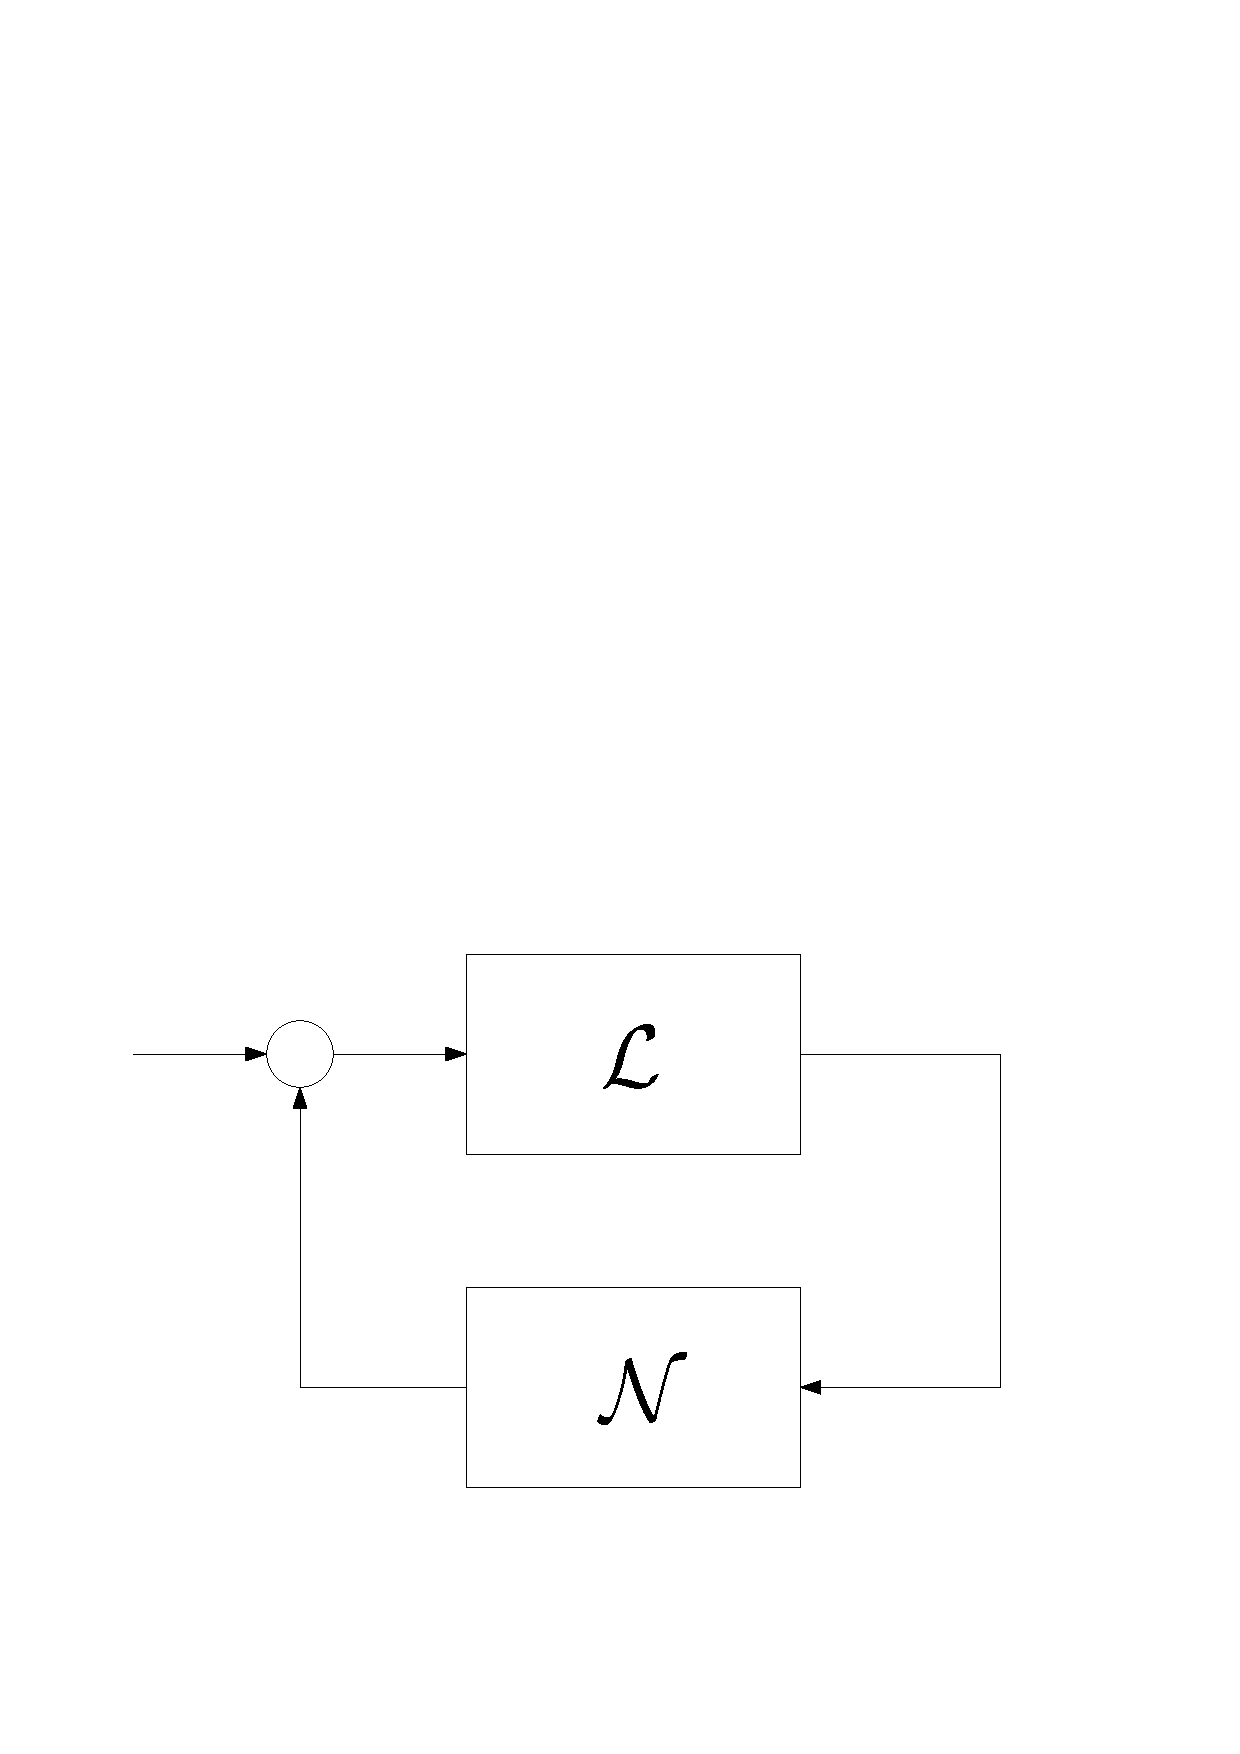
\includegraphics[width=0.4\columnwidth]{lure2}
		\end{figure}
	\begin{itemize}
		\item The system $\mathcal{L}$ can be fully described by its transfer function $G(s)$, that is the Laplace transform of its pulse response
		\item By ``memoryless block'' we mean an operator defined by a single-valued function $n(t,\cdot)$ (which can be time-varying)
	\end{itemize}
}

\frame{\frametitle{Lur'e systems (an example)}
	The classical pendulum equation is
	\begin{align}
		\ddot \theta + \beta \dot \theta + c\sin{\theta}= u(t)
	\end{align}
	which can be interpreted in terms of a Lur'e system
	\begin{figure}
		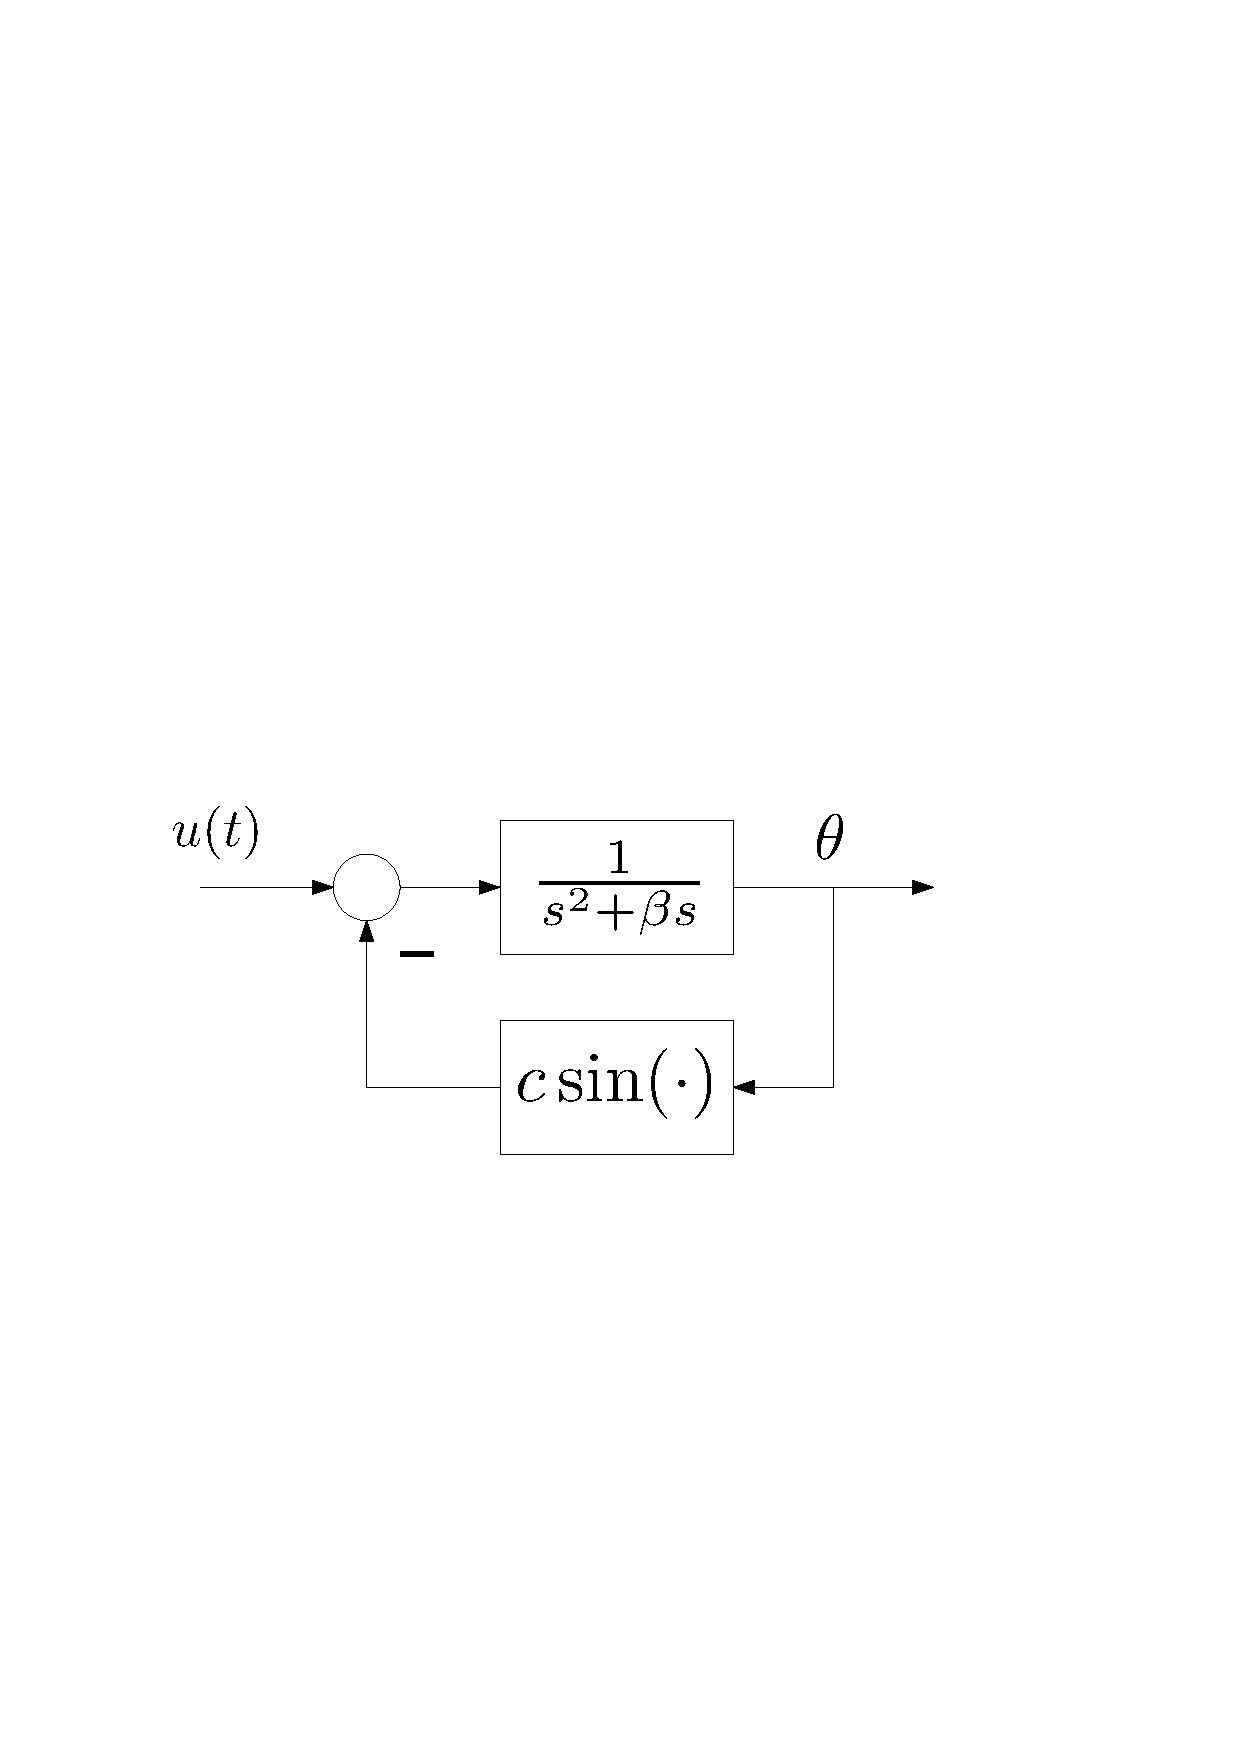
\includegraphics[width=0.6\columnwidth]{pendulum}
	\end{figure}
	The function $c\sin(\cdot)$ is a single-valued function that defines a ``memoryless'' block
}

\frame{\frametitle{The problem of Absolute Stability}
	In 1944, Lur'e and Postnikov formulated the following problem \cite{LurPos44}
	\smallskip
	\begin{block}{The Absolute Stability Problem}
		Given a LTI system $G(s)$, find the class of nonlinearities $n(t,\cdot)$ that makes the Lur'e interconnection Globally Asymptotically Stable
	\end{block}
	\begin{itemize}
		\item	The concept of Absolute Stability looks for a class of nonlinearities
		\item	It involves a direct notion of ``robustness''
	\end{itemize}
}

\frame{\frametitle{The Nyquist Criterion}
	First, let us consider the linear case.\\
	The only operators which are both linear and static are the constant gains.
% 	Then we deal with following system
	\begin{figure}
		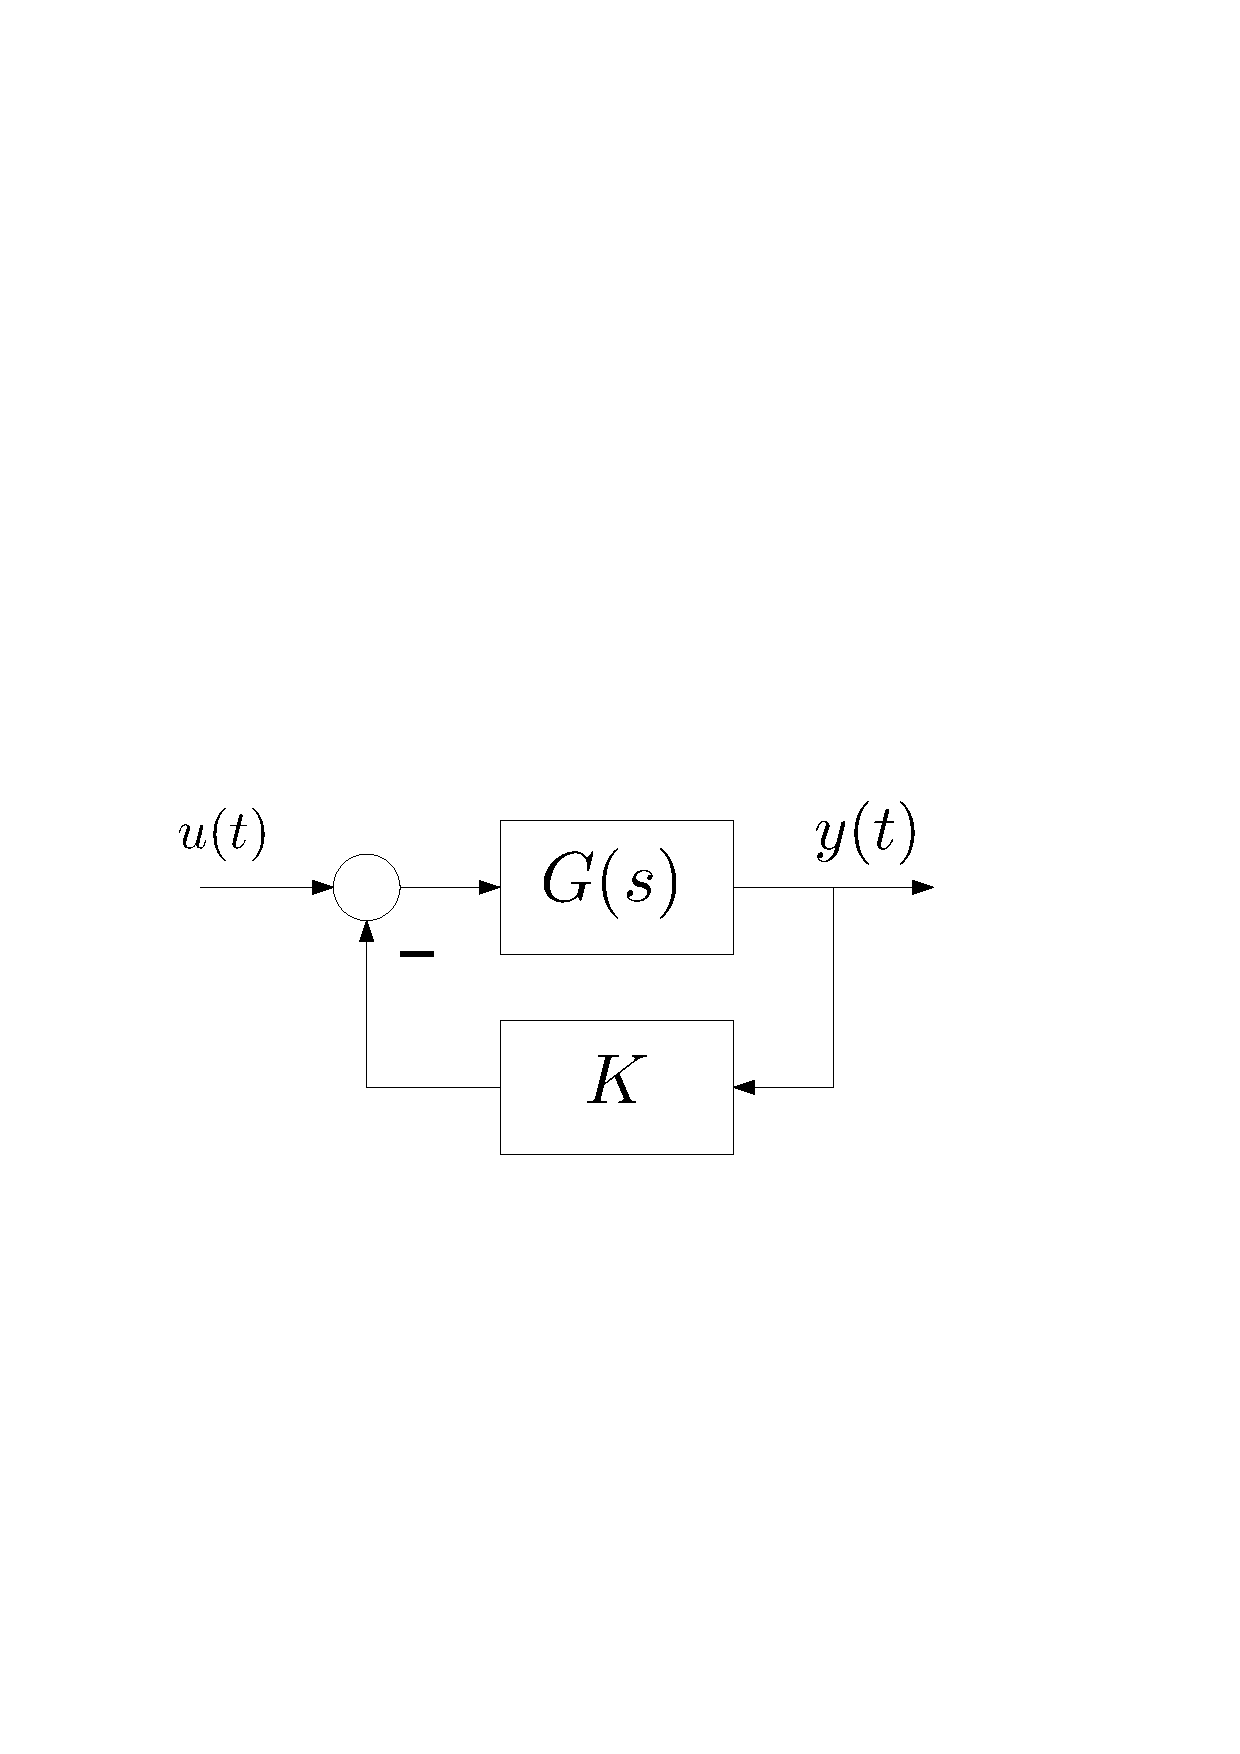
\includegraphics[width=0.4\columnwidth]{lure_linear}
	\end{figure}
% 	where $K$ is a simple multiplicative constant.
	\begin{block}{The Nyquist Criterion}
		The negative feedback of $G(s)$ with a proportional gain $K$ is stable iff the winding number of the curve $G(i\w)$ with respect to the point $-\frac{1}{K}$ is equal to the number unstable poles of $G(s)$.
	\end{block}
}

\frame{\frametitle{The Nyquist Criterion}
	The Nyquist criterion has an appealing graphical interpretation
	\begin{figure}
		\centering
		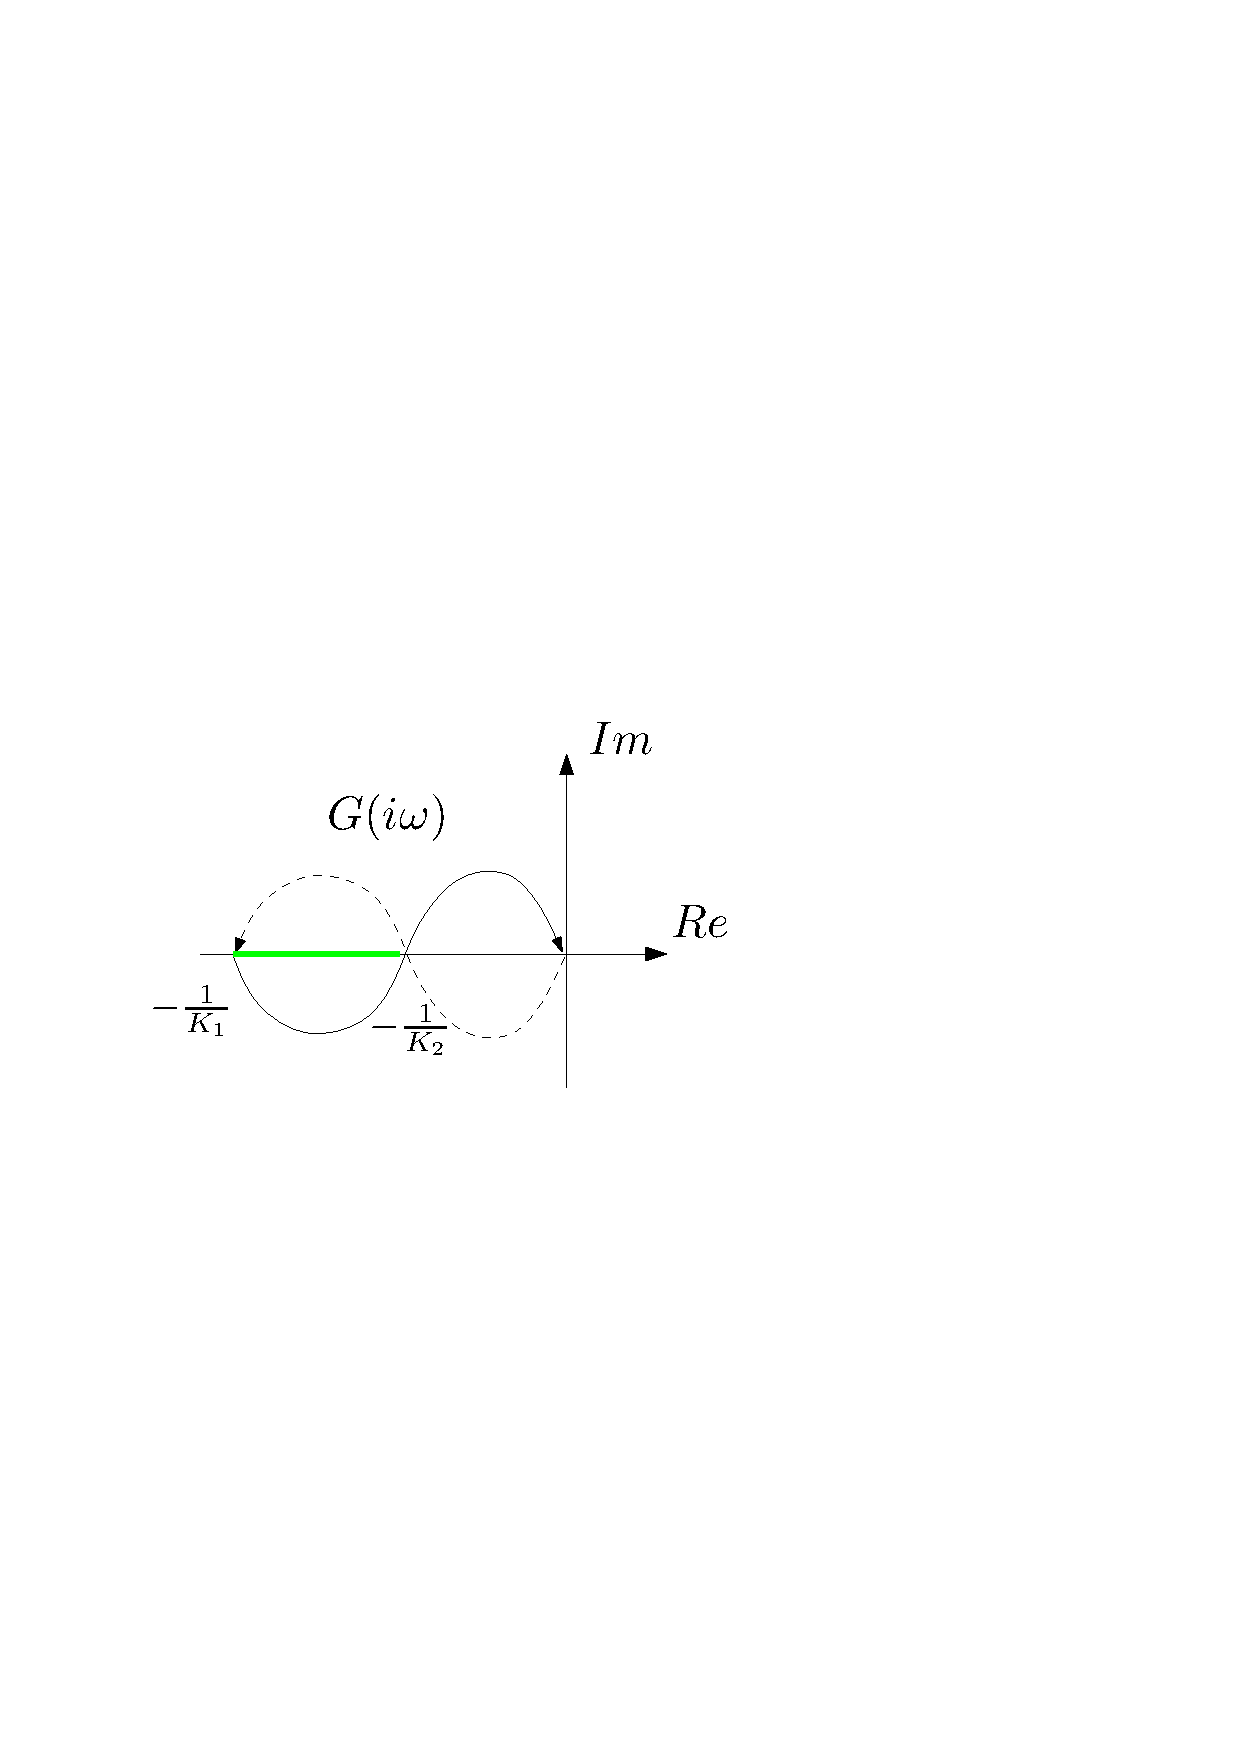
\includegraphics[width=0.5\columnwidth]{nyquist_hurwitz}
		\caption{Nyquist Plot of a transfer function with one unstable pole and two stable ones}
	\end{figure}
	\begin{itemize}
		\item The interval of values $[K_1, K_2]$ making the feedback interconnection stable is called ``Hurwitz sector''
		\item The area defined by the points with winding number equal the number of instability is called ``Hurwitz region''
	\end{itemize}
}

\frame{\frametitle{Sector Nonlinearities}
	We say that a memoryless operator $n(t,\cdot)$ belongs to the linear sector $[\alpha, \beta]$ if and only if it satisfies the relation
	\begin{align}
		0\leq (n(t,y)-\alpha y)(\beta y - n(t,y)) \qquad \text{for all } t,y
	\end{align}
	Graphically this means that
	\begin{figure}
		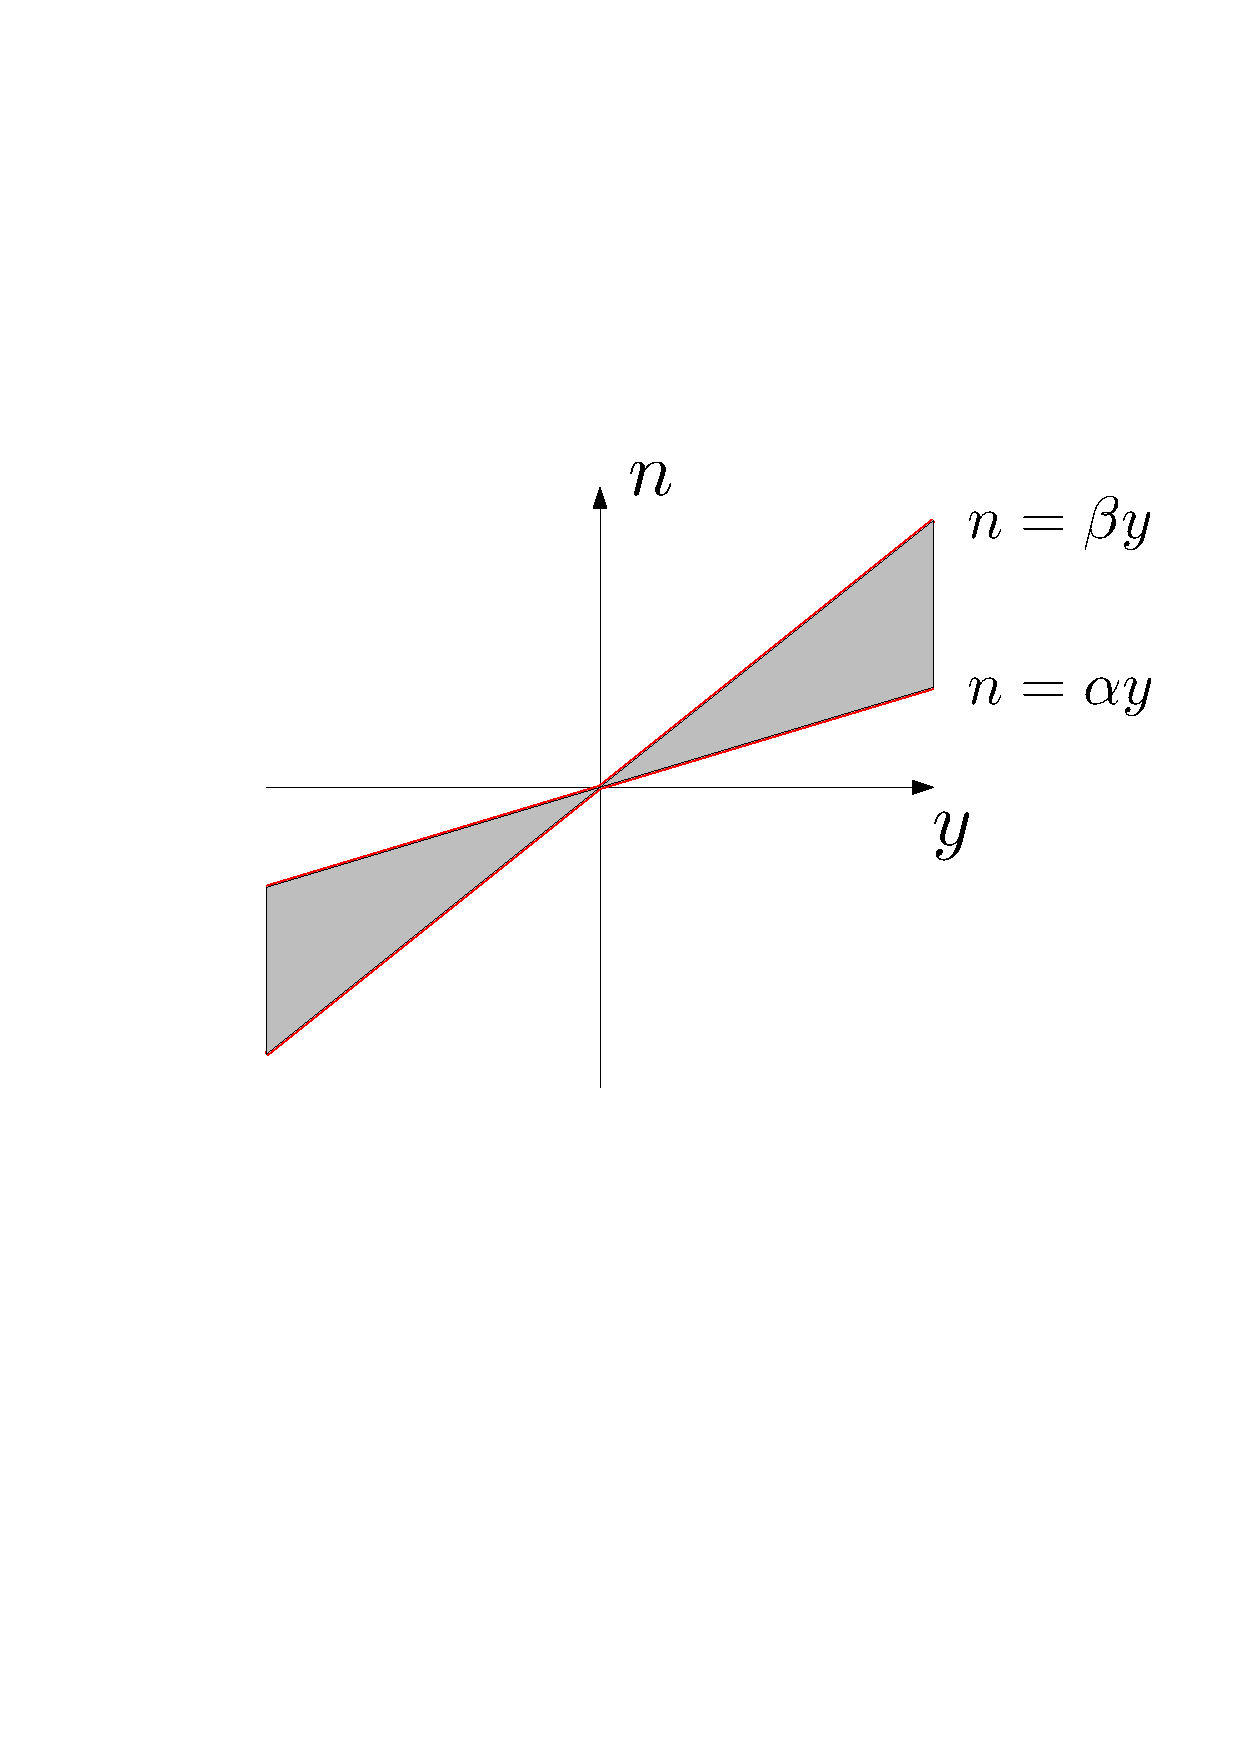
\includegraphics[width=0.4\columnwidth]{sectornonlin}
	\end{figure}
	the function $n(t,y)$ lies in the gray area beetween the two lines $n=\alpha y$ and $n=\beta y$.
}

\subsection{Conjectures about Absolute Stability}
\frame{\frametitle{The Aizerman and Kalman Conjectures}
	Aizerman stated the following conjecture
	\begin{block}{Aizerman Conjecture}
		If the feedback interconnection of $G(s)$ with $K$ is stable for any $K$ such that $\alpha \leq K \leq \beta$, then Lur'e system is stable for any $n(t,y)$ belonging to the sector $[\alpha, \beta]$.
	\end{block}
	\begin{itemize}
		\item	The Aizerman conjecture is false (in general)
	\end{itemize}

	Kalman stated the following conjecture
	\begin{block}{Kalman Conjecture}
		If the feedback interconnection of $G(s)$ with $K$ is stable for any $K$ such that $\alpha \leq K \leq \beta$, then Lur'e system is stable for any $n(t,y)$ such that
		\begin{align}
			\alpha \leq \frac{\partial}{\partial y}n(y) \leq \beta
		\end{align}
	\end{block}
	\begin{itemize}
		\item	The Kalman conjecture is false (in general)
	\end{itemize}
}

% \frame{\frametitle{The Kalman Conjecture}
% }

\section{Sufficient conditions for Absolute Stability}

\subsection{The Circle Criterion}
\frame{\frametitle{The Circle Criterion}
	Sufficient conditions for the stability of a Lur'e system are given by a very important result formulated for the first time in 1966 and referred to as the ``Circle Criterion'' \cite{Zam66b}.
	\begin{block}{Circle Criterion}
		The Lur'e system is stable for a nonlinearity $n$ if the two following conditions are met
		\begin{itemize}
			\item	$n$ belongs to a sector $[\alpha, \beta]$
			\item	the circle with diameter $[-1/\alpha, -1/\beta]$ is contained in the Hurwitz region of the Nyquist plot of $G(i\w)$
		\end{itemize}
	\end{block}
	\begin{figure}
		\centering
		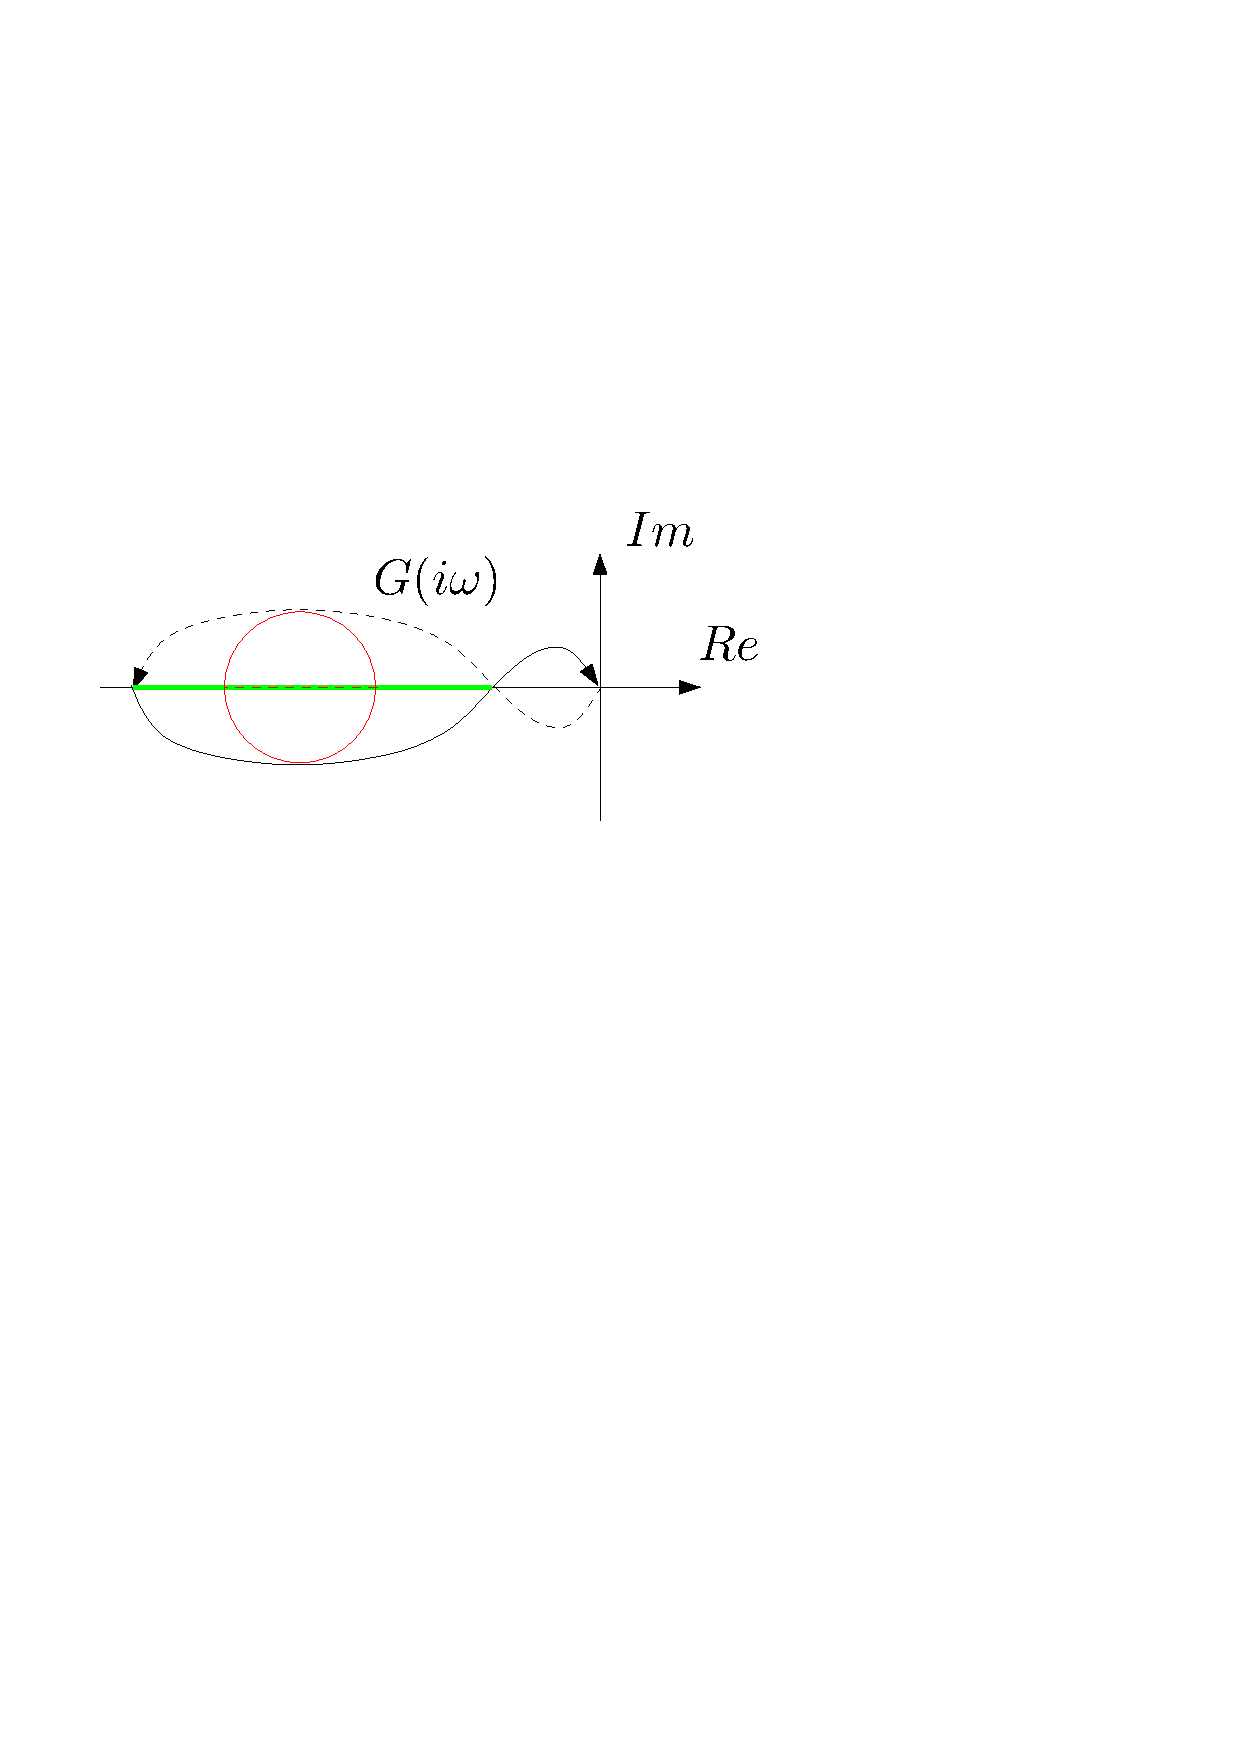
\includegraphics[width=0.6\columnwidth]{nyquist_circle}
	\end{figure}
}

\subsection{The solution based on IQC's/LMI's}
\frame{\frametitle{The Circle Criterion}
	\begin{block}{}
	The solution given by the Circle Criterion
	\begin{itemize}
		\item generalizes the Nyquist Criterion (the circle collapses into a point in the linear case)
		\item is very appealing for its graphical interpretation
		\item unfortunately is only a sufficient (and conservative) condition
	\end{itemize}
	\end{block}
	\smallskip
	\begin{itemize}
	\item  Following the Circle Criterion, many other criteria have been formulated in order to reduce its conservativeness
	\item A more general and systematic approach to Absolute Stability has been provided more recently using Integral Quadratic Constraints (IQC's) and Linear Matrix Inequalities (LMI's) \cite{MegRan97}
	\end{itemize}
}

\frame{\frametitle{Integral Quadratic Constraints}
	\begin{block}{Integral Quadratic Constraints}
	An operator $n$ satisfies an IQC defined by its ``multiplier'' $\Pi(i\w)$ if and only if, for any function $y(t) \in L_2$
	\begin{align}\nonumber
		& \int_{-\infty}^{+\infty}
			\left(\begin{array}{c}
				\hat y\\
				\hat{n}(y)
			\end{array}\right)^*
			\Pi(i\w)
			\left(\begin{array}{c}
				\hat y\\
				\hat{n}(y)
			\end{array}\right)
		d\w \geq 0.
	\end{align}
	where $\Pi(i\w)$ is a hermitian and uniformly bounded function of $\w$ and the $\hat{(\cdot)}$ denotes the Fourier transform.
	\end{block}
	\smallskip
	\begin{itemize}
		\item A sector condition can be formulated via IQC's in a easy way
		\item Using IQC's it is possible to formulate many other conditions on the operator $n(\cdot)$
		\item In the IQC formulation $n(\cdot)$ is an operator (it may have memory)
		\item IQC's can be extended to consider vector operators
	\end{itemize}
}

\frame{\frametitle{An IQC/LMI formulation}
	The following result gives a sufficient condition for absolute stability \cite{MegRan97}
	\begin{block}{IQC formulation}
		The Lur'e system is stable for a nonlinear operator $n$ if the two following conditions are met
		\begin{itemize}
			\item	$n$ satisfies the IQC with multiplier $\Pi(i\w)$
			\item
			\begin{equation}
				\left(\begin{array}{c}
					G(i\w)\\ I
				\end{array}\right)^*
				\Pi(i\w)
				\left(\begin{array}{c}
					G(i\w)\\ I
				\end{array}\right)
				<-\eps G^*(i\w)G(i\w)
			\end{equation}
		\end{itemize}
		for some $\eps>0$.
	\end{block}
	\begin{itemize}
		\item The first condition is a way to describe a nonlinearity class
		\item The second condition can be numerically checked using an LMI (generalized Kalman-Yacubovich-Popov lemma \cite{Ran96})
		\item This criterion provides a \textbf{unified framework} for almost all the other Absolute  Stability criteria
	\end{itemize}
}

\frame{\frametitle{The Circle Criterion in the IQC formulation}
	The Circle Criterion (along with many other absolute stability criteria) becomes a special case of the previous theorem
	\smallskip
	\begin{itemize}
		\item	the sector condition is equivalent to the IQC with multiplier
		\begin{align}
			\Pi(i\w)=
			\left(
				\begin{array}{cc}
					-\alpha\beta & \frac{\alpha+\beta}{2}\\
					\frac{\alpha+\beta}{2} & -1
				\end{array}
			\right)
		\end{align}
		Indeed we have that
		\begin{align*}
			0\leq
			(n-\alpha y)(\beta y -n)=
			\left(\begin{array}{c}
				y\\
				{n}(y)
			\end{array}\right)^T
			\left(
				\begin{array}{cc}
					-\alpha\beta & \frac{\alpha+\beta}{2}\\
					\frac{\alpha+\beta}{2} & -1
				\end{array}
			\right)
			\left(\begin{array}{c}
				y\\
				{n}(y)
			\end{array}\right)
		\end{align*}
		which leads to
		\begin{align}\nonumber
			& \int_{-\infty}^{+\infty}
				\left(\begin{array}{c}
					\hat y\\
					\hat{n}(y)
				\end{array}\right)^*
				\left(
					\begin{array}{cc}
						-\alpha\beta & \frac{\alpha+\beta}{2}\\
						\frac{\alpha+\beta}{2} & -1
					\end{array}
				\right)
				\left(\begin{array}{c}
					\hat y\\
					\hat{n}(y)
				\end{array}\right)
			d\w \geq 0.
	\end{align}
	\end{itemize}
}

\frame{\frametitle{The Circle Criterion in the IQC formulation}
	About the second condition, the following three statements are equivalent
\begin{itemize}
		\item  the circle with diameter $[-1/\alpha, -1/\beta]$ is inside the Hurwitz region of the curve $G(i\w)$
		\item for some $\eps>0$
		\begin{equation}
			\left(\begin{array}{c}
				G(i\w)\\ I
			\end{array}\right)^*
			\left(
				\begin{array}{cc}
					-\alpha\beta & \frac{\alpha+\beta}{2}\\
					\frac{\alpha+\beta}{2} & -1
				\end{array}
			\right)
			\left(\begin{array}{c}
				G(i\w)\\ I
			\end{array}\right)
			<-\eps G^*(i\w)G(i\w)
		\end{equation}
		\item the following LMI has solution with respect to $P=P^T>0$ and $r>0$
		\begin{equation*}
			\small
			\left(
				\begin{array}{cc}
					A^T P +P A +rP & PB\\
					B^T P & 0
				\end{array}
			\right)+
			\left(\begin{array}{cc}
				C & 0\\
				0 & I
			\end{array}\right)^T
			\left(\begin{array}{cc}
				-\alpha\beta & \frac{\alpha+\beta}{2}\\
				\frac{\alpha+\beta}{2} & -1
			\end{array}\right)
			\left(\begin{array}{cc}
				C & 0\\
				0 & I
			\end{array}\right)<0
		\end{equation*}
		where $(A, B, C, 0)$ is any minimal realization of the strictly proper transfer function $G(s)$.
\end{itemize}
}

\frame{\frametitle{Comments on the results}
	Let us try to summarize the main points
	\begin{itemize}
		\item We have defined the class of Lur'e systems
		\item The problem of Absolute Stability has been formulated
		\item Some conjectures have been stated, but they are not true
		\item A first (conservative) solution is given by the Circle Criterion
		\item There is a powerful generalization which is given by the IQC/LMI formulation of the problem
	\end{itemize}
	\smallskip
	Let us try to introduce a technique to reduce the conservativeness of these criteria
}

\section{Less Conservative conditions for Absolute Stability}

\subsection{A less conservative Circle Criterion}
\frame{\frametitle{A weak form of the Circle Criterion}
	We introduce a weaker formulation of the Circle Criterion proving boundedness of the state trajectories [Materassi \& Salapaka, 2006]
% 	\cite{MatSal06}
	\begin{block}{Weak Circle Criterion}
		Consider a Lur'e system whose linear part has transfer function $G(s)$ minimally realized by $(A,B,C,0)$ and output $y$.
		Assume that the two following conditions are met
		\begin{itemize}
			\item	$-M \leq (n-\alpha y)(\beta y -n)$
% 			\item	the circle with diameter $[-1/\alpha, -1/\beta]$ is contained in the Hurwitz region of the nyquist plot of $G(i\w)$.
			\item the following LMI has solution $P>0$, $r>0$
			\begin{equation*}
			\small
			\left(\begin{array}{cc}
				A^T P +P A +rP & PB\\
				B^T P & 0
			\end{array}\right)+
			\left(\begin{array}{cc}
				-\alpha\beta C^T C & \frac{\alpha+\beta}{2}C^T\\
				\frac{\alpha+\beta}{2}C & -1
			\end{array}\right)<0
			\end{equation*}
		\end{itemize}
		Then, the ellipsoid 
% 		there is a constant $\gamma>0$ such that the output $y$ of the system satisfies
		\begin{align}
			\ellips_P\left(\frac{M}{r}\right)\doteq \left\{x|x^T P x \leq \frac{M}{r} \right\}
		\end{align}
		is a globally attracting and positively invariant set for the system trajectories
% 		\begin{align}
% 			y(t)^2 \leq \frac{M}{r}C^TP^{-1}C \qquad \text{for t ``large enough''}
% 		\end{align}
	\end{block}
	\smallskip
% 	This result is different form the Circle Criterion only on the first condition which introduces a \textbf{bias term} on the quadratic constraint.
}

\frame{\frametitle{A weak form of the Circle Criterion}
	\begin{figure}
		\centering
		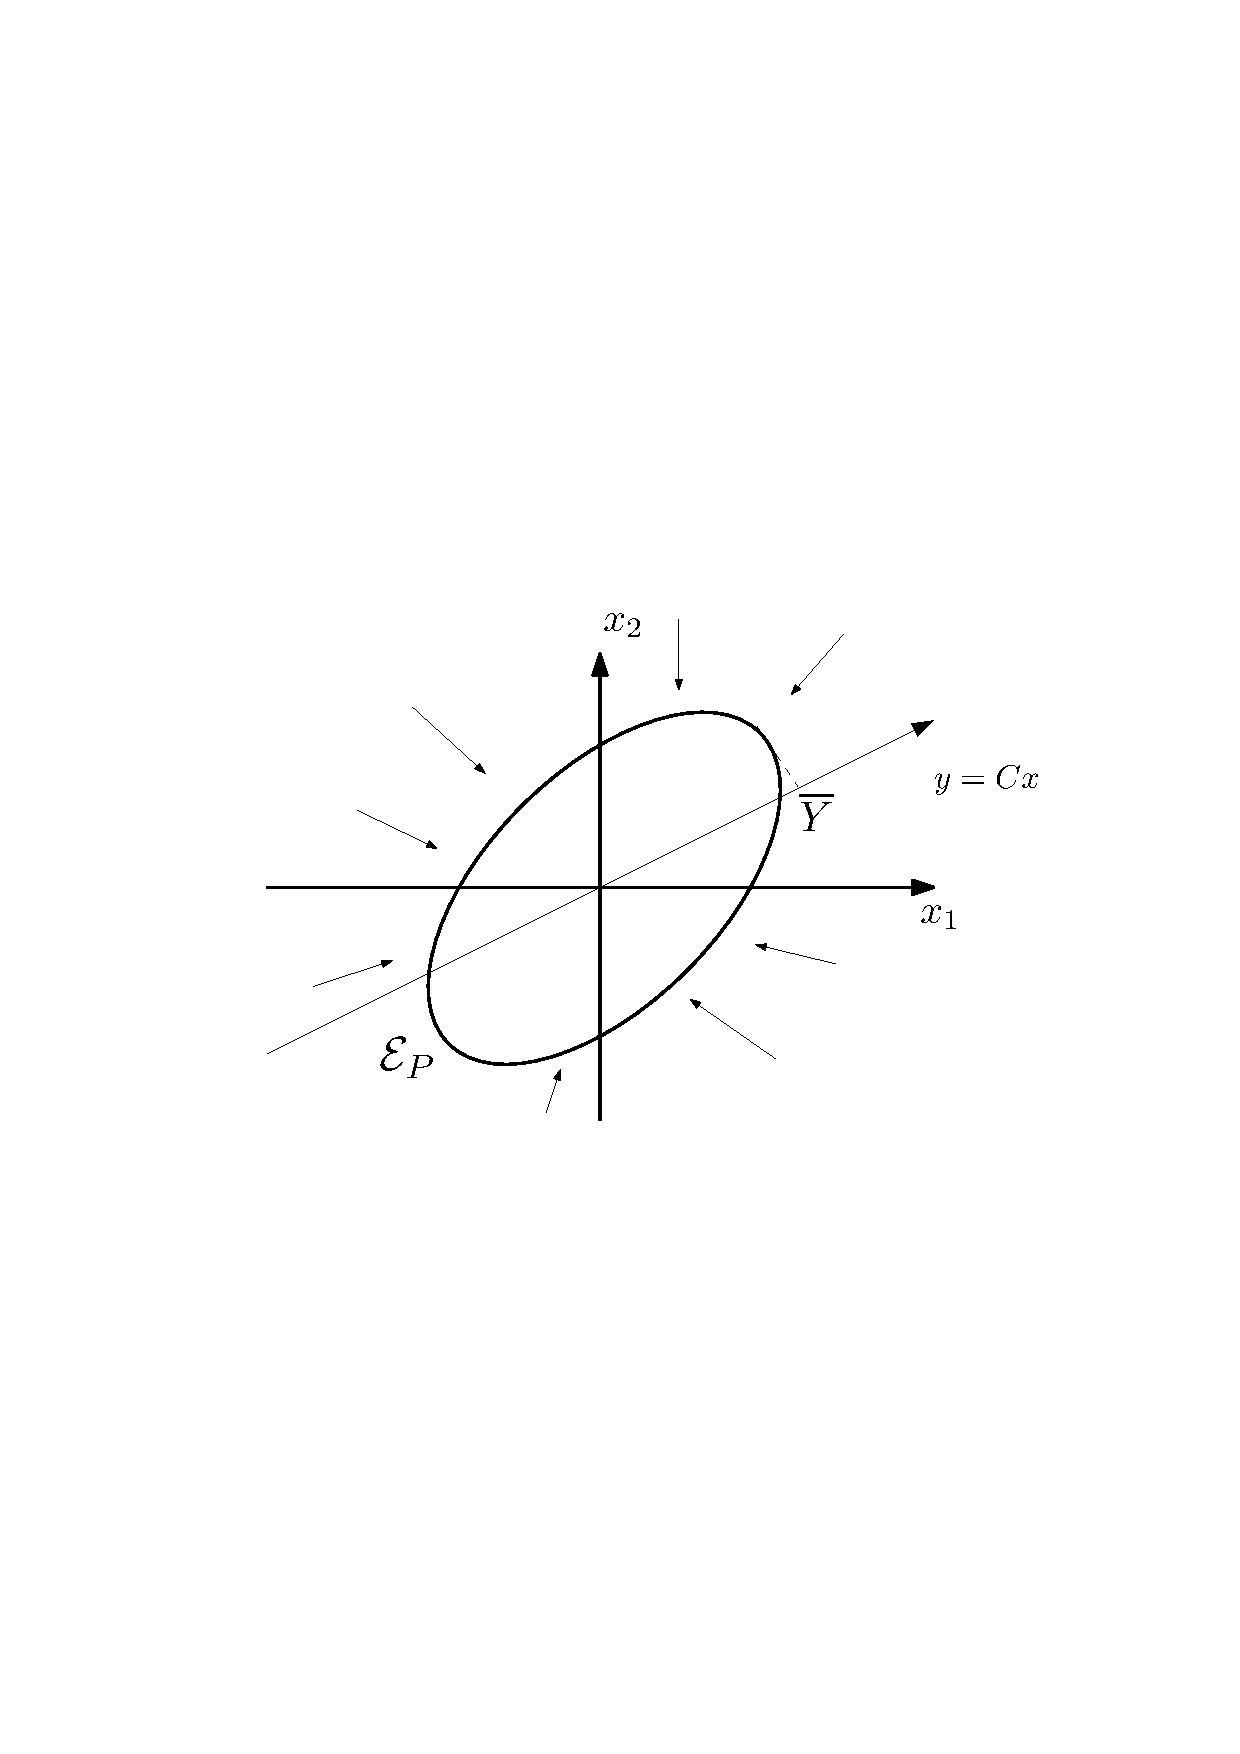
\includegraphics[width=0.5\columnwidth]{Bottle}
		\caption{Phase portrait with the positively invariant ellipsoid $\mathcal{E}_P(M/r)$}
	\end{figure}

	As a corollary we have
	\begin{block}{Corollary}
		Under the assumptions of the Weak Circle Criterion
		\begin{align}
			y(t)^2 \leq \overline{Y}^2 \doteq \frac{M}{r}C^TP^{-1}C \qquad \text{for t ``large enough''}
		\end{align}
	\end{block}
}


\frame{\frametitle{Hyperbolic Sectors}
	We have introduced a bias term in the quadratic constraint defining the linear sector condition.
	Let us see what this
	\begin{align}
		-M \leq (n-\alpha y)(\beta y -n)
	\end{align}
	means in graphical terms.
	\smallskip
	We can say that it describes a ``hyperbolic sector''
	\begin{figure}
		\centering
		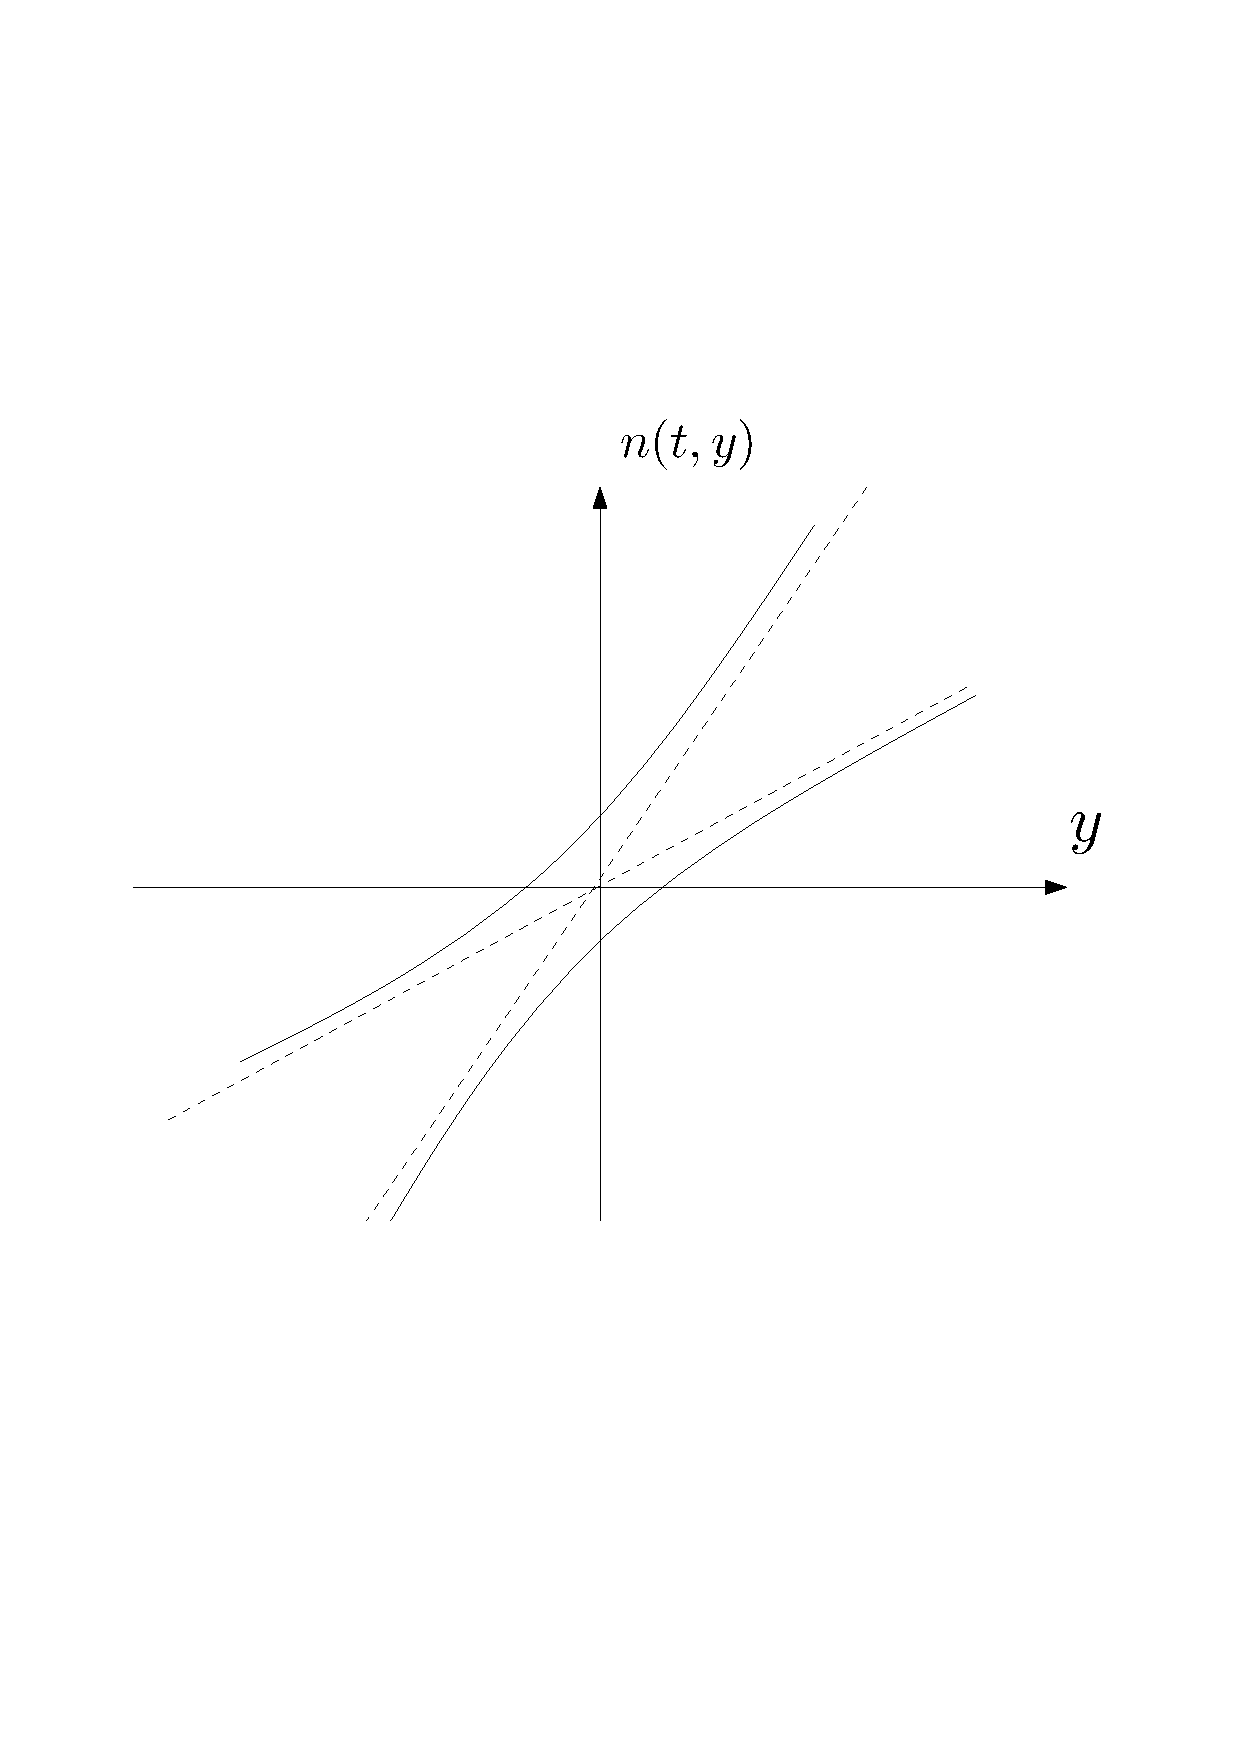
\includegraphics[width=0.5\columnwidth]{hypersector2}
	\end{figure}
}

\frame{\frametitle{A weak form of the Circle Criterion}
	We can draw the following considerations
	\begin{itemize}
		\item	The presence of a bias term in the quadratic constraint of the Circle Criterion leads to the definition of nonlinearities lying in a hyperbolic-sector
		\item	A hyperbolic-sector nonlinearity is similar to a linear sector nonlinearity for a large $|y|$ 
		\item	Conversely the nonlinearity is very free around the origin (we do not even need the existence of an equilibrium)
		\item	The weak Circle Criterion is a tool to conclude practical stability about a Lur'e system
	\end{itemize}
	\smallskip
	Can we exploit the weak circle criterion to obtain less conservative conditions for Absolute Stability?
}

\frame{\frametitle{Less conservative conditions for AS}
	\begin{figure}
		\centering
		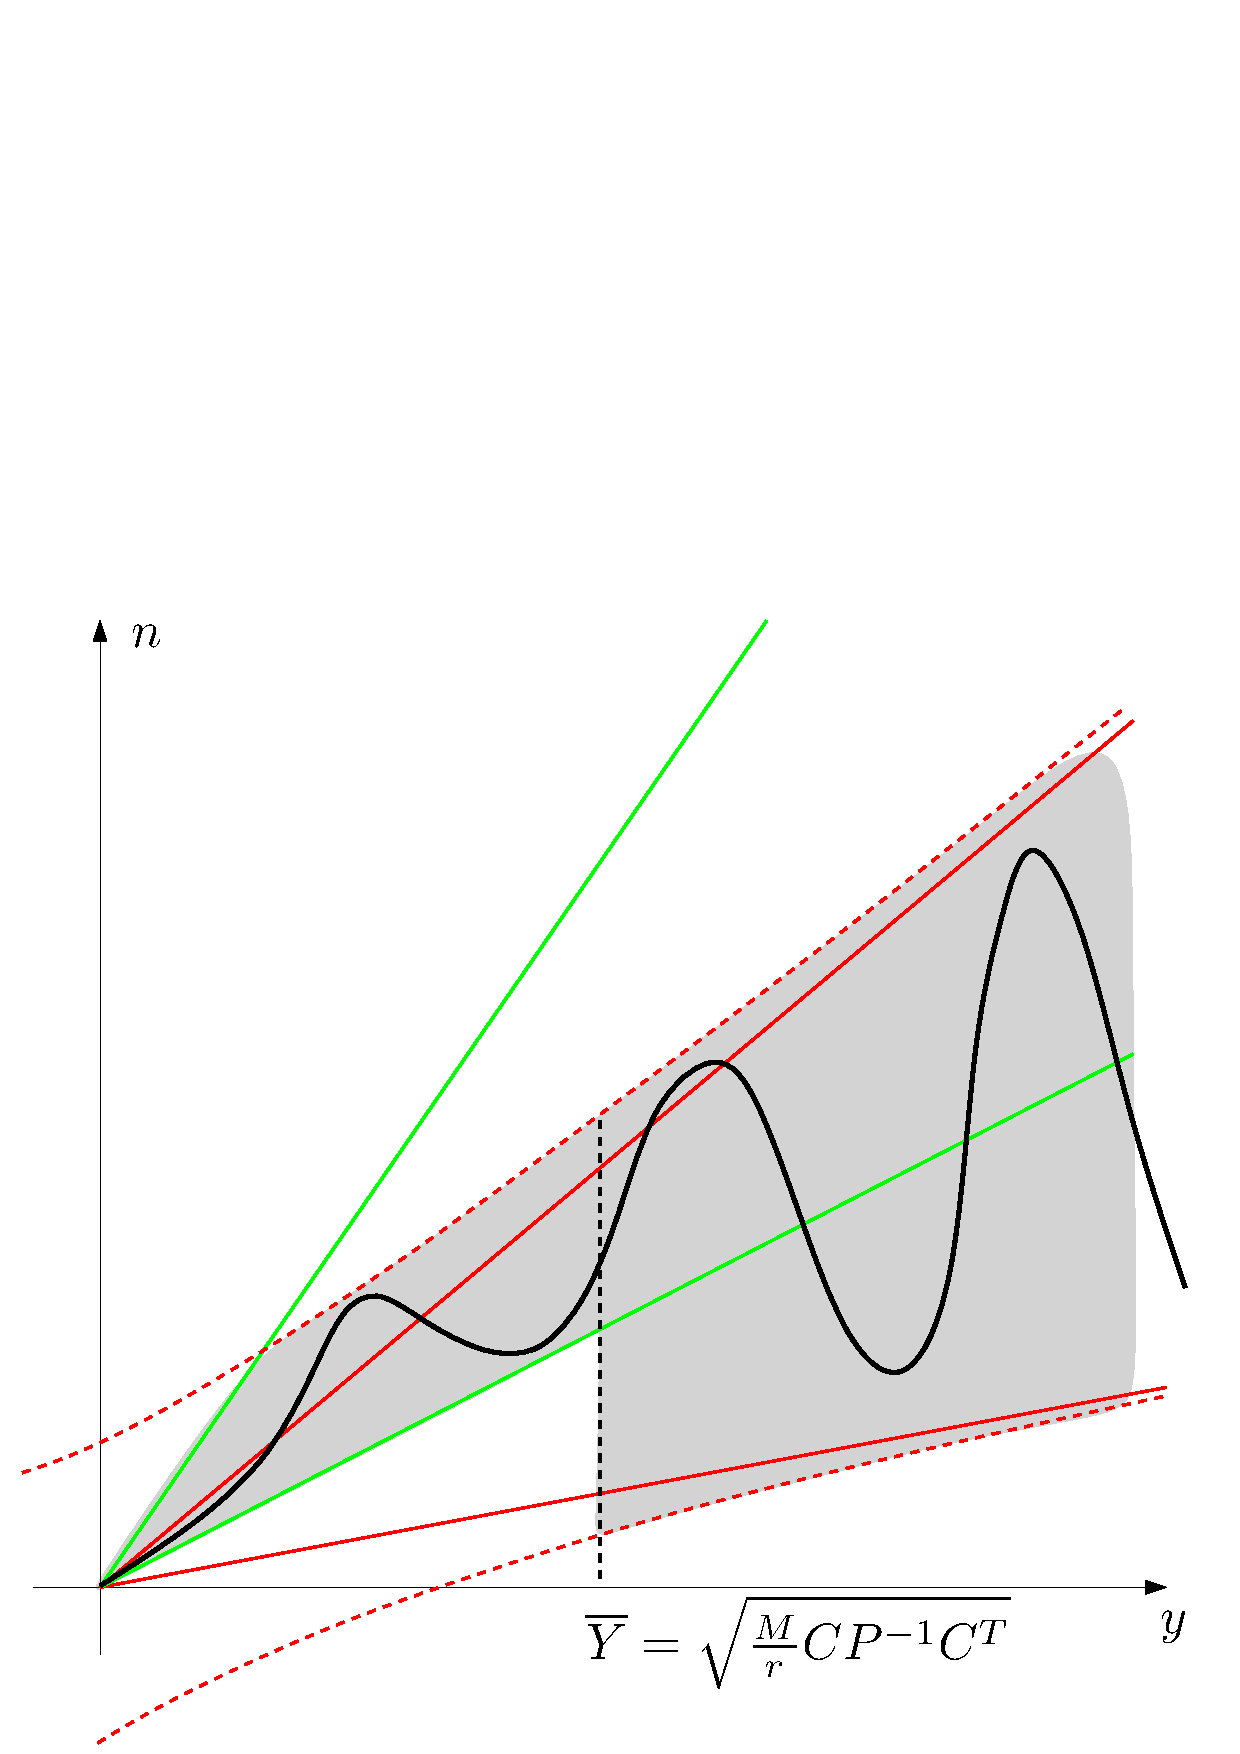
\includegraphics[width=0.6\columnwidth]{doublesector}
	\end{figure}
	The boundedness condition provided by the hyperbolic sector (red) can be exploited to restrict the region of the nonlinearity which is explored ($|y|<\overline{Y}$). Then, a linear sector condition (green) can be applied to conclude stability.
}

\frame{\frametitle{Less conservative conditions for AS}
	Using the previous consideration, the sector of stability can be enlarged combining two (or more) ``circles'' \cite{MatSal06}
	\begin{figure}
		\centering
		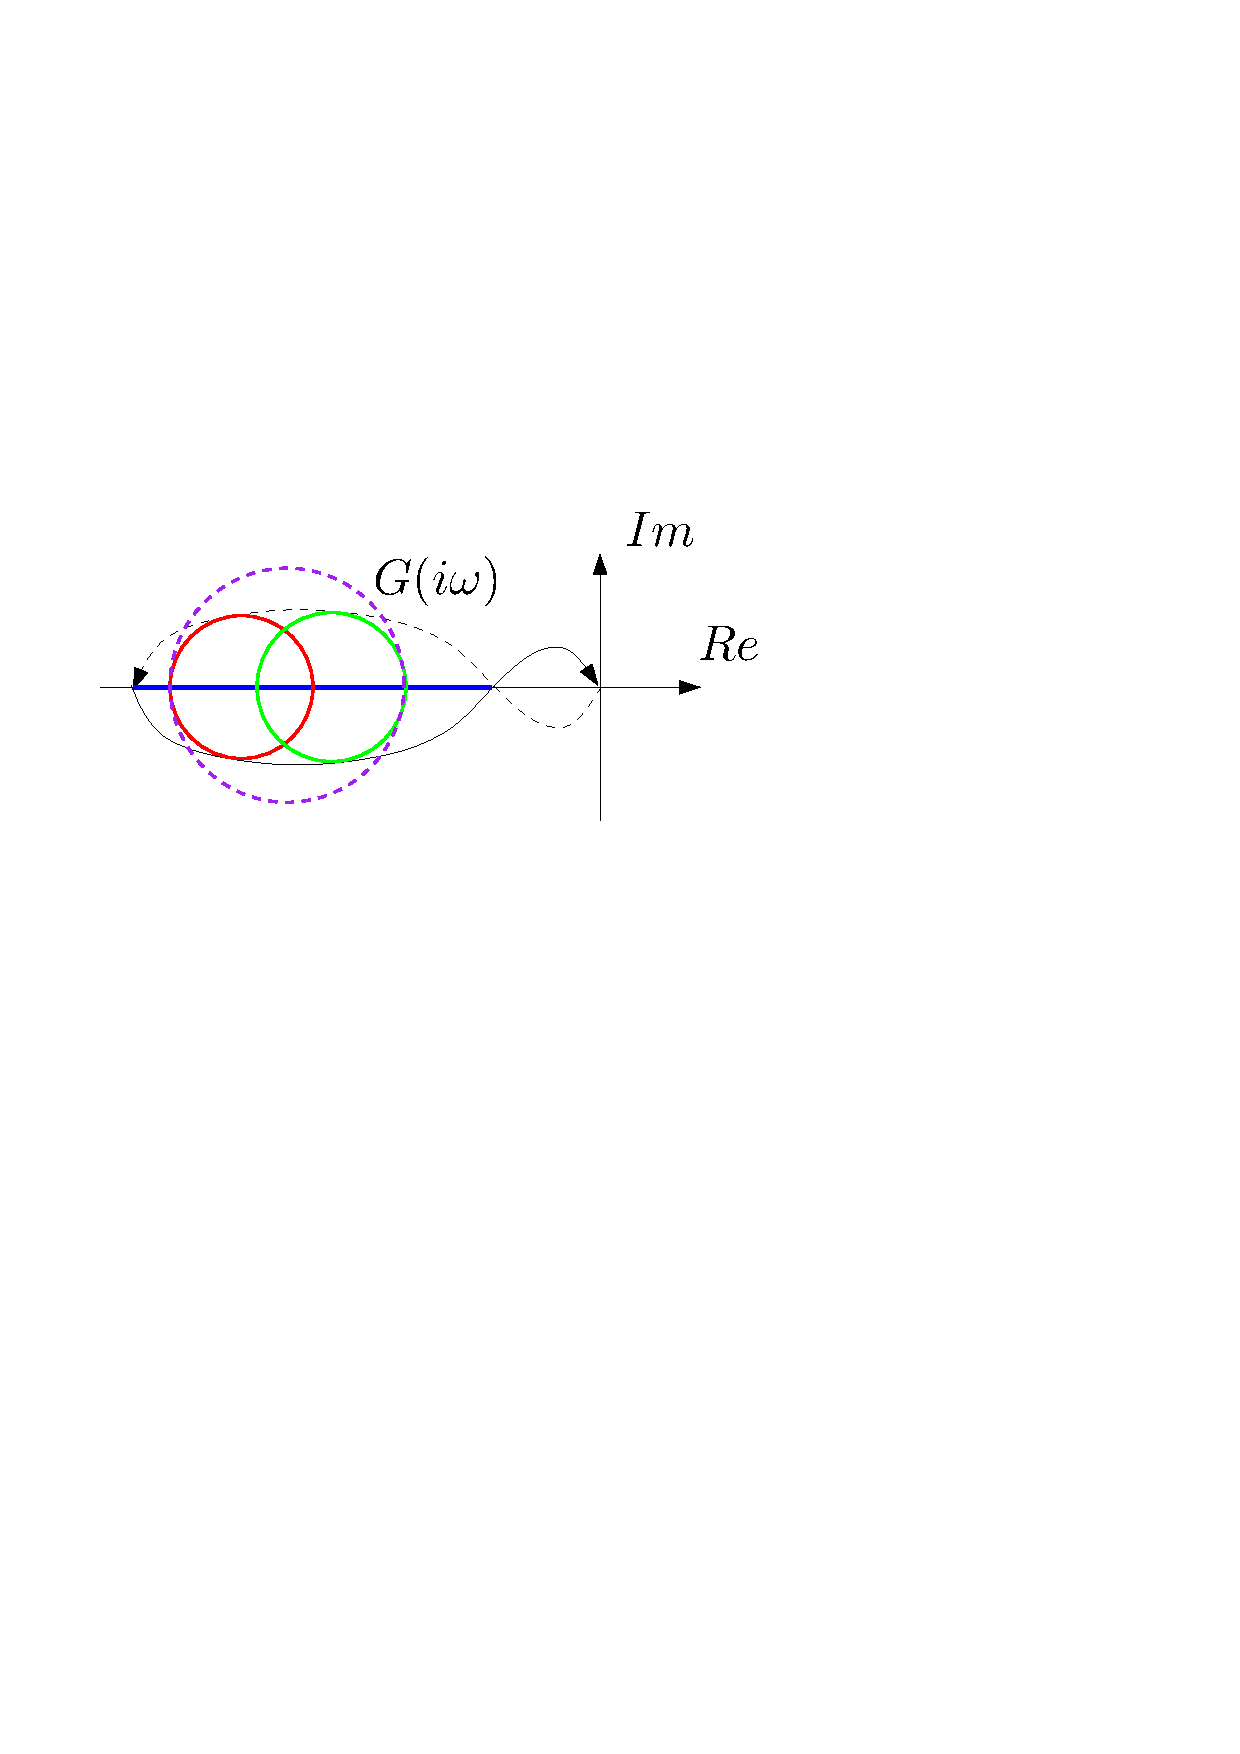
\includegraphics[width=0.6\columnwidth]{nyquist_doublecircle}
		\caption{If a nonlinearity spans a large linear sector (purple circle) the Circle Criterion can not be applied. However, if the nonlinearity lies in a hyperbolic sector (i.e. the red circle), then the region where it is explored can be restricted. If the restricted region lies in a smaller linear sector (i.e. the green circle) , the circle criterion can be applied}
	\end{figure}
}

\frame{\frametitle{Less conservative conditions for AS}
	We can state the following result
	\begin{block}{Theorem}
		Let $S$ be a Lur'e system made of a SISO linear block with a strictly proper transfer function $G(s)$ (minimally realized by $(A,B,C,0)$ ) and  nonlinear static block $n(t,y)$. Let $\alpha_1<\beta_1, \alpha_2<\beta_2$ be four scalars. Assume that	%\renewcommand{\labelenumi}{(\textit{\alph{enumi}})}
		\begin{enumerate}
% 			\item The sectors $[\alpha_1, \beta_1]$ and $[\alpha_2, \beta_2]$ are in the Hurwitz region of $G(i\w)$
			\item the following LMI's have solutions $P_i>0$, $r_i>0$ ($i=1,2$)
			\begin{equation*}
			\small
			\left(\begin{array}{cc}
				A^T P_i +P_i A +r_iP_i & PB\\
				B^T P_i & 0
			\end{array}\right)+
			\left(\begin{array}{cc}
				-\alpha_i\beta_i C^T C & \frac{\alpha_i+\beta_i}{2}C^T\\
				\frac{\alpha_i+\beta_i}{2}C & -1
			\end{array}\right)<0
			\end{equation*}
			\item there exists $M_1>0$ such that 
			\begin{equation} 
				-M_1\leq (n(t,y)-\alpha_1 y)(\beta_1 y - n(t,y)) \nonumber
			\end{equation}
			\item $\|y(t)\|_{\infty}^2<\frac{M_1}{r_1}C^TP_1C$ implies
				\qquad $0\leq\ (n(t,y)-\alpha_2 y)(\beta_2 y - n(t,y))$
		\end{enumerate}
		Then we can conclude Global Asymptotic Stability for the system.	
	\end{block}
}

\frame{\frametitle{Less conservative conditions for AS}
	Nothing forbids to apply the procedure with more than one hyperbolic sector
	\begin{block}{Theorem}
		Let $S$ be a Lur'e system made of a SISO linear block with a strictly proper transfer function $G(s)$ and  nonlinear static block $n(t,y)$. Let $\alpha_i<\beta_i$ be $2N$ scalars. Assume that	%\renewcommand{\labelenumi}{(\textit{\alph{enumi}})}
		\begin{enumerate}
% 			\item The sectors $[\alpha_1, \beta_1]$ and $[\alpha_2, \beta_2]$ are in the Hurwitz region of $G(i\w)$
			\item the following LMI's have solutions $P_i>0$, $r_i>0$ ($i=1,...,N$)
			\begin{equation*}
			\small
			\left(\begin{array}{cc}
				A^T P_i +P_i A +r_iP_i & PB\\
				B^T P_i & 0
			\end{array}\right)+
			\left(\begin{array}{cc}
				-\alpha_i\beta_i C^T C & \frac{\alpha_i+\beta_i}{2}C^T\\
				\frac{\alpha_i+\beta_i}{2}C & -1
			\end{array}\right)<0
			\end{equation*}
			\item there exists $M_1>0$ such that 
			\begin{equation} 
				-M_1\leq (n(t,y)-\alpha_1 y)(\beta_1 y - n(t,y)) \nonumber
			\end{equation}
			\item $\|y(t)\|_{\infty}^2<\frac{M_i}{r_i}C^TP_iC$ implies
				$-M_{i+1}\leq\ (n(t,y)-\alpha_{i+1} y)(\beta_{i+1} y - n(t,y))$
			\item $M_N=0$
		\end{enumerate}
		Then we can conclude Global Asymptotic Stability for the system.	
	\end{block}
}

\subsection{A less conservative IQC's/LMI's formulation}
\frame{\frametitle{A less conservative IQC/LMI formulation}
	\begin{itemize}
		\item the introduction of a \textbf{bias term} in the quadratic constraint of the Circle Criterion has allowed one to enlarge the class of nonlinearities which provide asymptotic stability for the system
		\item the previous considerations about the Circle Criterion can be suitably modified in order to be applied to the IQC/LMI case
		\item we intend to generalize the concept of IQC in order to include a bias term in its formulation
		\item the way to accomplish this goal is not trivial
		\begin{itemize}
			\item the bias term in the Circle Criterion occurs in a quadratic constraint formulated in the time domain
			\item IQC's deal with $L_2$ signals, thus we will need to formulate the constraints in order to take into account $L_{2e}$ signals
		\end{itemize}
	\end{itemize}
}

% \frame{\frametitle{Local Quadratic Constraints}
% 	In order to generalize the IQC definition, let us start from a special case of IQC's, that is Local Quadratic Constraints
% 	\begin{block}{Local Quadratic Constraint}
% 		Given a constant matrix $\Sigma\geq 0$, we define the quadratic form $\sigma: \Re^n \times \Re^n \rightarrow \Re$
% 		\begin{equation}\nonumber
% 			\sigma(y,u)=
% 					\left(\begin{array}{c}
% 						y\\
% 						u
% 					\end{array}\right)^*
% 					\Sigma
% 					\left(\begin{array}{c}
% 						y\\
% 						u
% 					\end{array}\right).
% 		\end{equation}
% 		We say that a nonlinear operator $n(\cdot)$ satisfies the Local Quadratic Constraint (LQC) defined by $\sigma$, if and only if
% 		\begin{equation}\label{eq:defLQC}
% 			\sigma(y(t),n(y(t)))\geq 0 \qquad \text{for all}~t>0
% 		\end{equation}
% 		for any signal $y(t)\in L_{2}$.
% 	\end{block}
% 	Note that if a LQC is satisfied, by integration we immediately obtain that an IQC is satisfied.
% }
% 
% \frame{\frametitle{Biased Local Quadratic Constraint}
% 	The introduction of a 
% }


\frame{\frametitle{Static IQC's}
	When the multiplier $\Pi(i\w)=\Sigma$ of an IQC does not depend on the frequency $\w$, the IQC is said ``static''
	\begin{align}\nonumber
		& \int_{-\infty}^{+\infty}
			\left(\begin{array}{c}
				\hat y\\
				\hat{n}(y)
			\end{array}\right)^*
			\Sigma
			\left(\begin{array}{c}
				\hat y\\
				\hat{n}(y)
			\end{array}\right)
		d\w \geq 0.
	\end{align}
	and the Parseval theorem allows an immediate ``translation'' into the time domain
	\begin{align}\nonumber
		& \int_{0}^{+\infty}
			\left(\begin{array}{c}
				y(t)\\
				n(y(t))
			\end{array}\right)^T
			\Sigma
			\left(\begin{array}{c}
				y(t)\\
				n(y(t))
			\end{array}\right)
		dt \geq 0.
	\end{align}
	We generalize an IQC introducing a bias term $M$ in the following way
	\begin{align}\nonumber
		& \liminf_{T\rightarrow +\infty}
		\int_{0}^{T}
			\left[
			\left(\begin{array}{c}
				y(t)\\
				n(y(t))
			\end{array}\right)^T
			\Sigma
			\left(\begin{array}{c}
				y(t)\\
				n(y(t))
			\end{array}\right)+M
			\right]
		dt \geq 0.
	\end{align}
}

\frame{\frametitle{Biased IQC's (static case)}
	This motivates the following definition
	\begin{block}{Biased (static) Integral Quadratic Constraint}
		A nonlinear operator $n(\cdot)$ satisfies a Biased (static) IQC  defined by $\Sigma$ with bias $M>0$ if and only if
		\begin{equation}\label{eq:biqc_condition}
			\liminf_{T\rightarrow +\infty}
			\int_{0}^{T}
				\left[
				\left(\begin{array}{c}
					y(t)\\
					n(y(t))
				\end{array}\right)^T
				\Sigma
				\left(\begin{array}{c}
					y(t)\\
					n(y(t))
				\end{array}\right)+M
				\right]
			dt \geq 0.
		\end{equation}
	We also use $n \in BIQC(\Sigma,M)$, if $n$ satisfies the condition
	\end{block}
}

\frame{\frametitle{A ``weak'' IQC/LMI criterion}
	This result is analogous to the theorem we have seen for the Weak Circle Criterion
	\begin{block}{Theorem}
	Consider a Lur'e system $\mathcal{S}$.\\
	Let its linear part $G(s)$ be a strictly proper transfer function minimally realized by $(A,B,C,0)$ with state $x$.
	Suppose that
	\begin{itemize}
		\item $n\in BIQC(\Sigma,M)$ with
		\item there exists a solution $(P, r)$ to the following LMI
			\begin{equation*}
			\left(\begin{array}{cc}
				A^T P +P A +rP & PB\\
				B^T P & 0
			\end{array}\right)+
			\left(\begin{array}{cc}
				C & 0\\
				0 & I
			\end{array}\right)^T
			\Sigma
			\left(\begin{array}{cc}
				C & 0\\
				0 & I
			\end{array}\right)
			<0
			\end{equation*}
		with $P=P^T$, $P>0$, $r \in \mathcal{R}^+$,
	\end{itemize}
	then, there exists $\overline{t}$ such that $t>\overline{t}$ implies $x(t)\in \ellips_P(M/r)$ and $|y(t)|^2 < MCP^{-1}C^T/r$
	\end{block}
}


\frame{\frametitle{A two-step stability result}
	This result is the equivalent of the 2-step procedure we have already introduced with the Circle Criterion
	\begin{block}{Theorem}
		Let $S$ be a Lur'e system made of a SISO linear block with a strictly proper transfer function $G(s)$ realized by $(A,B,C,0)$ and  nonlinear static block $n(t,y)$. Assume that
		\begin{enumerate}
% 			\item The sectors $[\alpha_1, \beta_1]$ and $[\alpha_2, \beta_2]$ are in the Hurwitz region of $G(i\w)$
			\item the following LMI's have solutions $P_i>0$, $r_i>0$ ($i=1,2$)
			\begin{equation*}
			\left(\begin{array}{cc}
				A^T P_i +P_i A +r_iP_i & PB\\
				B^T P_i & 0
			\end{array}\right)+
			\left(\begin{array}{cc}
				C & 0\\
				0 & I
			\end{array}\right)^T
			\Sigma_i
			\left(\begin{array}{cc}
				C & 0\\
				0 & I
			\end{array}\right)
			<0
			\end{equation*}
			\item $n\in BIQC(\Sigma_1,M_1)$
			\item $\|y(t)\|_{\infty}^2<\frac{M_1}{r_1}C^TP_1C$ implies
				$n\in BIQC(\Sigma_2,0)$
		\end{enumerate}
		Then we can conclude Global Asymptotic Stability for the system.	
	\end{block}	
}

\frame{\frametitle{A $N$-step stability result}
	And this is the corresponding $N-$step procedure
	\begin{block}{Theorem}
		Let $S$ be a Lur'e system made of a SISO linear block with a strictly proper transfer function $G(s)$ realized by $(A,B,C,0)$ and  nonlinear static block $n(t,y)$. Assume that
		\begin{enumerate}
% 			\item The sectors $[\alpha_1, \beta_1]$ and $[\alpha_2, \beta_2]$ are in the Hurwitz region of $G(i\w)$
			\item the following LMI's have solutions $P_i>0$, $r_i>0$ ($i=1,...,N$)
			\begin{equation*}
			\small
			\left(\begin{array}{cc}
				A^T P_i +P_i A +r_iP_i & PB\\
				B^T P_i & 0
			\end{array}\right)+
			\left(\begin{array}{cc}
				C & 0\\
				0 & I
			\end{array}\right)^T
			\Sigma_i
			\left(\begin{array}{cc}
				C & 0\\
				0 & I
			\end{array}\right)
			<0
			\end{equation*}
			\item $n\in BIQC(\Sigma_1,M_1)$
			\item $\|y(t)\|_{\infty}<\frac{M_i}{r_i}C^TP_iC$ then
				$n\in BIQC(\Sigma_{i+1},M_{i+1})$
			\item $M_N =0$
		\end{enumerate}
		Then we can conclude Global Asymptotic Stability for the system.	
	\end{block}	
}

% \frame{\frametitle{Dynamic IQC's}
% 	In the more general case, where the multiplier $\Pi(i\w)$ of an IQC does depend on the frequency $\w$, the IQC is said ``dynamic''.\\
% 	It is always possible to reduce a dynamic IQC to a static IQC by introducing an additional dynamics.
% 	\begin{block}{}
% 		Let $\Pi(s)\in\mathcal{C}^{(p+m)\times(p+m)}$ be real rational and globally bounded on the imaginary axis $s=i\w$ with $\w\in\Re$ and $p,m\in \mathbb{N}$.
% 		Then, $\Pi(s)$ admits the following factorization
% 		\begin{equation}\label{eq:PIfactorization}
% 			\Pi(s)=
% 				\left(\begin{array}{cc}
% 					T_1(s)		& T_2(s)\\
% 					I_m		& 0 \\
% 					0		& I_p
% 				\end{array}\right)^*
% 				\Gamma
% 				\left(\begin{array}{cc}
% 					T_1(s)		& T_2(s)\\
% 					I_m		& 0 \\
% 					0		& I_p
% 				\end{array}\right)
% 		\end{equation}
% 		with $T(s):=(T_1(s) ~ T_2(s))$ proper, stable and minimum phase.
% 	\end{block}
% }

\frame{\frametitle{Dynamic IQC's}
	In the more general case, where the multiplier $\Pi(i\w)$ depends on the frequency $\w$, it is always possible to reduce the ``dynamic'' IQC to a static IQC by introducing an additional dynamics.
	\begin{block}{}
		Given a standard dynamic IQC in the form
		\begin{align}\label{eq:dynIQCform}
			& \int_{-\infty}^{+\infty}
				\left(\begin{array}{c}
					\hat y\\
					\hat n
				\end{array}\right)^*
				\Pi(i\w)
				\left(\begin{array}{c}
					\hat y\\
					\hat n
				\end{array}\right)
			d\w \geq 0
		\end{align}
		defined by a real rational and bounded matrix $\Pi(i\w)$, then there exist a constant matrix $\Sigma$ and a stable, minimum phase and strictly proper transfer function $G_{\pi}(s)$ such that (\ref{eq:dynIQCform}) implies
		\begin{equation*}
			\int_{0}^{+\infty}
				\left(\begin{array}{c}
					y_{\pi}\\ y\\ n\\
				\end{array}\right)^T
				\Sigma
				\left(\begin{array}{c}
					y_{\pi}\\ y\\ n\\
				\end{array}\right)
			d\tau \geq 0
		\end{equation*}
		where
		\begin{equation}
			y_{\pi}=G_{\pi}(s)\left(\begin{array}{c}
						y\\ n(y)
					\end{array}\right)
		\end{equation}
	\end{block}
}

\frame{\frametitle{Biased Integral Quadratic Constraint}
	The previous result motivates the following definition
	\begin{block}{Biased Integral Quadratic Constraint}
		Consider a minimum phase, stable, linear time-invariant system with transfer function $G_{\pi}(s)$.
		We say that a nonlinear operator $n$ satisfies the BIQC with auxiliary dynamics $G_{\pi}(s)$ defined by a matrix $\Sigma$ with bias $M>0$ if and only if
		\begin{equation}
		\liminf_{T\rightarrow +\infty}
			\int_0^{~T}
				\left[
				\left(\begin{array}{c}
					y_{\pi}\\ y\\ n\\
				\end{array}\right)^T
				\Sigma
				\left(\begin{array}{c}
					y_{\pi}\\ y\\ n\\
				\end{array}\right)+M
				\right]
			d\tau\geq 0
		\end{equation}
		where
		\begin{equation}
			y_{\pi}=G_{\pi}(s)\left(\begin{array}{c}
						y\\ n(y)
					\end{array}\right).
		\end{equation}
		As a notation we write that $n(\cdot) \in BIQC(G_{\pi}(s),\Sigma,M)$.
	\end{block}
}

\frame{\frametitle{The augmented system}
	Consider a Lur'e system $\mathcal{S}$ described by a strictly proper transfer function $G(s)$ and a non linear operator $n\in BIQC(G_{\pi}(s),\Sigma,M)$.
	Let $x_G(0)$ be the initial state of $G(s)$.\\
	Consider a minimal realization $(A_G, B_G, C_G, 0)$ of $G(s)$ and a minimal realization $(A_{\pi}, B_{\pi}, C_{\pi}, 0)$ of the auxiliary dynamics $G_{\pi}(s)$.
	Decompose $B_{\pi}$ as
	\begin{equation}
		B_{\pi}=\left( \begin{array}{cc} B_y & B_{n} \end{array}\right).
	\end{equation}
	We define the ``augmented system'' as the Lur'e system $S_e$ with output $y_e$ given by the feedback interconnection of $G_e(s)=C_e(sI-A_e)^{-1}B_e$ with state $x_e$ and the non linear operator $n_e$ where
	\begin{align*}
		& A_e=
		\left(\begin{array}{cc}
			A_{\pi}	& B_y C_G\\
			0	& A_G
		\end{array}\right),
		& B_e=
		\left(\begin{array}{c}
			B_{n}\\
			B_G
		\end{array}\right),\\
		& C_e=
		\left(\begin{array}{cc}
			C_{\pi}	& 0\\
			0	& C_G
		\end{array}\right),
		& D_e=
		\left(\begin{array}{c}
			0\\
			0
		\end{array}\right),\\
		& x_e(0)=
			\left(\begin{array}{cc}
				0\\
				x_G (0)\\
			\end{array}\right),
		& y_e=C_e x_e,\\
		& n_e(y_e)=n([0~I]y_e).
	\end{align*}
}

\frame{\frametitle{The augmented system}
	\begin{block}{The augmented system}
		Consider a Lur'e system $S$ given by the interconnection of a strictly proper transfer function $G(s)$ and a non linear operator $n\in BIQC(G_{\pi}(s),\Sigma,M)$.\\
		\smallskip
		Consider its augmented system $S_e$ as in previous definition. Then, for all $t$
		\begin{equation}\nonumber
			x_G(t)=[\begin{array}{ll} 0 &I \end{array}] x_e(t)
		\end{equation}
		and $n_e$ satisfies a static BIQC
		\begin{equation}\nonumber
			n_e \in BIQC(\Sigma,M)
		\end{equation}	
	\end{block}
	\begin{itemize}
		\item	Given a Lur'e system $\mathcal{S}$ such that its nonlinear operator $n\in BIQC(G_{\pi},\Sigma,M)$, it is always possible to define an augmented Lur'e system $\mathcal{S}_e$ with the same stability properties such that its nonlinear operator $n_e\in BIQC(\Sigma,M)$
	\end{itemize}

}

% \frame{\frametitle{A practical stability result}
% 	Let $G(s)$ be a strictly proper transfer function minimally realized by $(A,B,C,0)$. Consider the nonlinear operator $n(\cdot)$ such that
% 	\begin{equation}
% 		n(\cdot)\in BIQC(G_{\pi},\Sigma, M).
% 	\end{equation}
% 	Consider the ``augmented system'' $S_e$ as given by the previous definition.
% 	Decompose the matrix $\Sigma$ in such a way that
% 	\begin{equation*}
% 		\left(\begin{array}{c}
% 			y_{\pi}\\
% 			y\\
% 			n
% 		\end{array}\right)^T
% 		\Sigma
% 		\left(\begin{array}{c}
% 			y_{\pi}\\
% 			y\\
% 			n
% 		\end{array}\right)=
% 		\left(\begin{array}{c}
% 			y_e\\
% %			n_e
% 			n
% 		\end{array}\right)^T
% 		\left(
% 			\begin{array}{cc}
% 				Q	& S \\
% 				S^T	& R
% 			\end{array}
% 		\right)
% 		\left(\begin{array}{c}
% 			y_e\\
% %			n_e
% 			n
% 		\end{array}\right).
% 	\end{equation*}
% 	If there exists a solution $P>0, r>0$ to the following LMI
% 	\begin{equation}\label{eq:LMIextended}
% 		\left[
% 			\begin{array}{cc}
% 				A_e^TP+PA_e+C_e^TQC_e+rP	& PB_e+C_e^TS \\
% 				B_e^TP+S^TC_e			& R
% 			\end{array}
% 		\right] < 0
% 	\end{equation}
% 	then, there exists $\gamma$ (function of $C_e$, $r$ and $P$) such that
% 	\begin{equation}
% 		y(t)^2 \leq \gamma^2 M \qquad \text{for $t$ large enough}
% 	\end{equation}
% }

\section{A numerical example}
\frame{\frametitle{A numerical example}
	Let us consider the linear system $G(s)$ which was analyzed also in \cite{MegRan97}
	\begin{equation}
		G(s)=\frac{s^2}{s^3+2s^2+2s+1}
	\end{equation}
	Its Nyquist plot is shown in Figure \ref{fig:nyquist Megretski example}.
	\begin{figure}
		\centering
		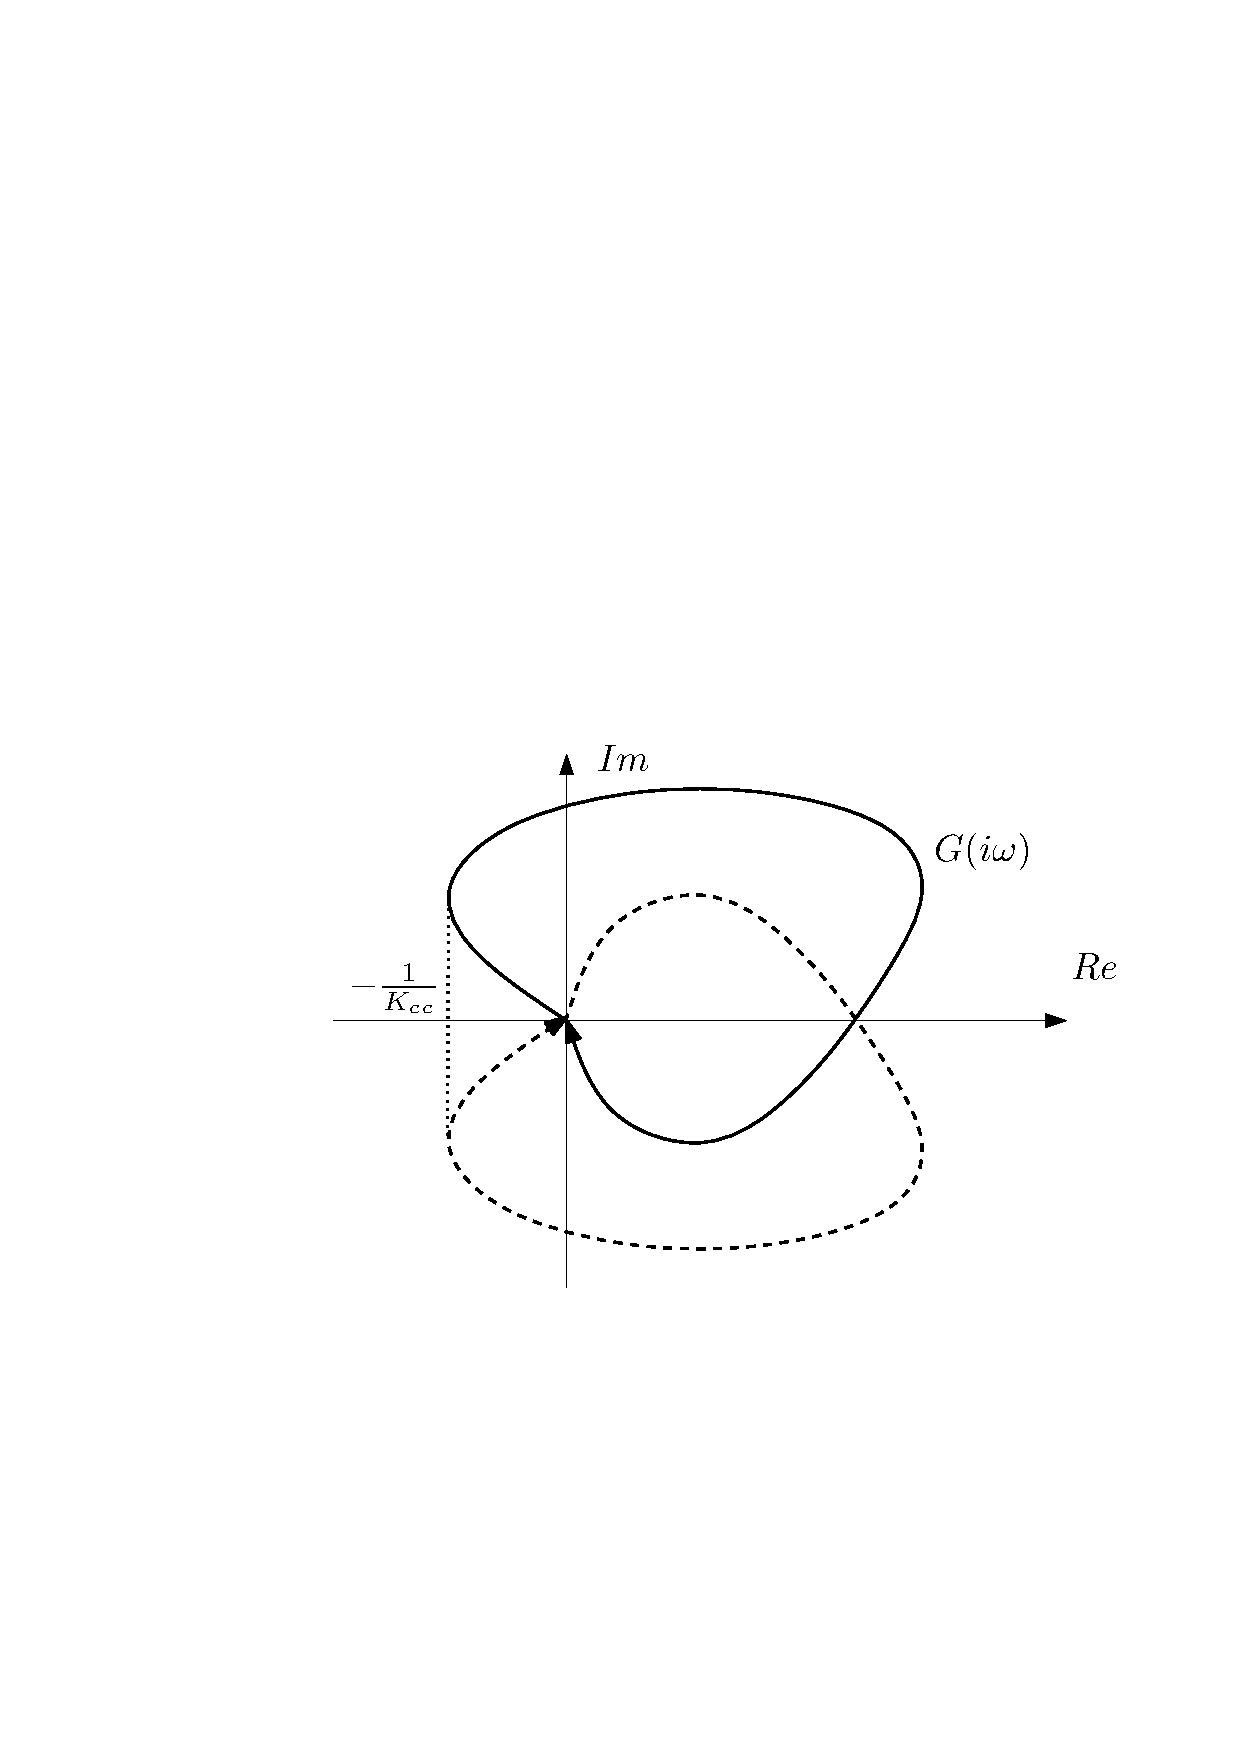
\includegraphics[width=0.6\columnwidth]{nyquist_MegreskiExample2}
		\caption{Nyquist plot of the transfer function $G(s)$\label{fig:nyquist Megretski example}}
	\end{figure}
}

\frame{\frametitle{A numerical example}
	We consider the transfer function $G(s)$ in feedback connection with the nonlinearity $n(t,y)=(1+\delta(y))\sat_A(ky)$
	\begin{figure}
		\centering
		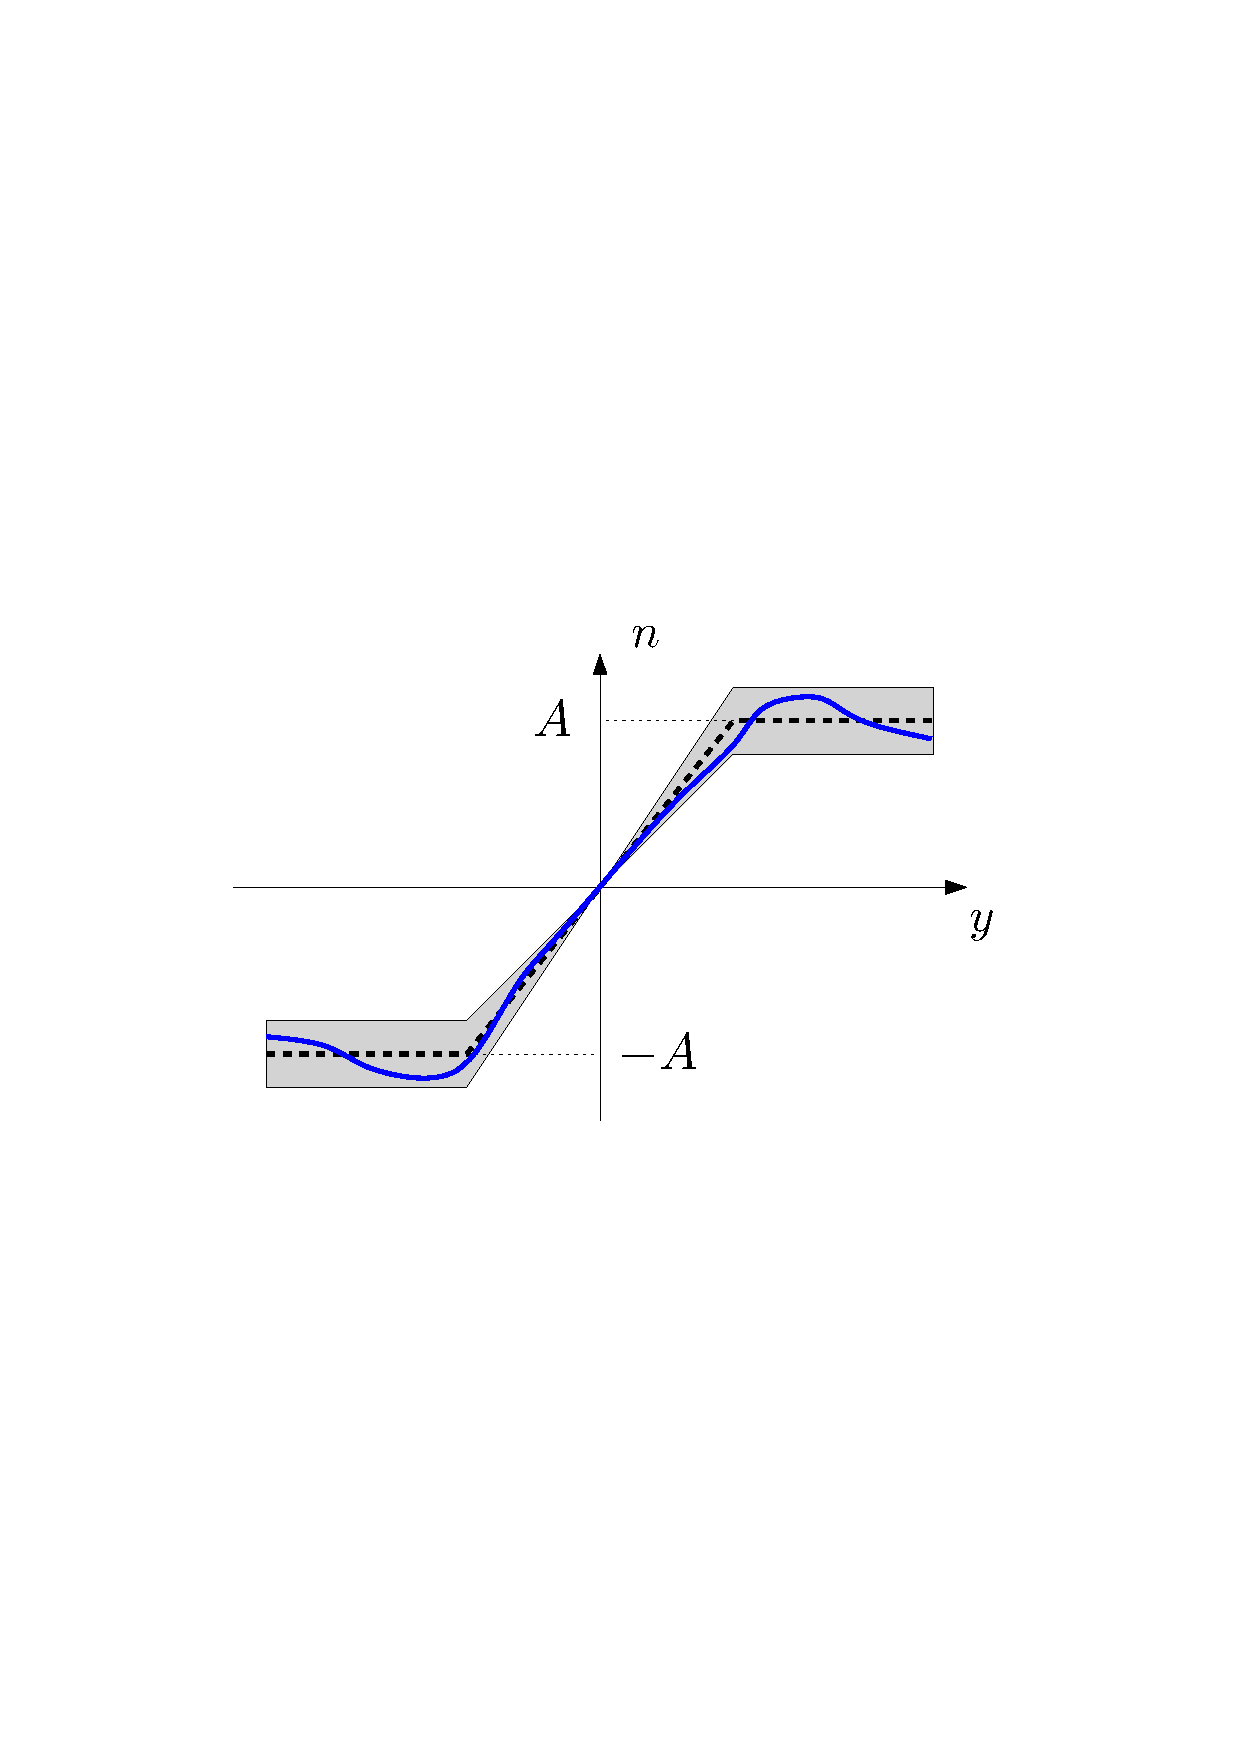
\includegraphics[width=0.6\columnwidth]{nonlinear_ex02}
		\caption{Saturation with uncertainty\label{fig:example}}
	\end{figure}
	where
	\begin{equation}
		\sat_A(z)=
			\left\{\begin{array}{ll}
				z & \quad \text{if}~|z|<A\\
				A & \quad \text{otherwise}
			\end{array}\right.
	\end{equation}
	and $|\delta(y)|\leq D\leq 1$ is a bounded relative uncertainty
}

% \frame{\frametitle{A numerical example}
% 	This scenario is more general than the scenario provided in \cite{MegRan97} where there is no uncertainty ($D=0$).
% 	We want to study how the parameter $k$ influences the stability of the system.
% 	It immediately follows that the nonlinearity $\Xi(\cdot)$ is in the sector $[0, k(1+D)]$. The application of the Circle Criterion provides a conservative result stating that the system is stable for
% 	\begin{equation}
% 		k(1+D)< k_{cc}\simeq 8.13.
% 	\end{equation}
% 	The Popov criterion improves the result by a small amount, guaranteeing stability for
% 	\begin{equation}
% 		k(1+D)< k_{pc}\simeq 8.90.
% 	\end{equation}
% }

% \frame{\frametitle{A numerical example}
% 	When there is no uncertainty ($D=0$), it would possible to exploit a powerful IQC found by Zames and Falb for monotonic and odd nonlinearities which guarantees stability for any positive value of $k$
% 	\begin{equation}
% 		\small
% 		\int_{-\infty}^{+\infty}
% 			\left(\begin{array}{c}
% 				\hat y(t) \\
% 				\hat n(t)
% 			\end{array}\right)^*
% 			\left(\begin{array}{cc}
% 				0 		& 1+\hat L(i\w)\\
% 				1+\hat H(-i\w)	& -2(1+ \text{Re}\{\hat H(i\w)\})/k
% 			\end{array}\right)
% 			\left(\begin{array}{c}
% 				\hat y(t) \\
% 				\hat n(t)
% 			\end{array}\right)
% 		dt \geq 0
% 	\end{equation}
% 	where $H(s)$ is any transfer function such that its $L_1$ norm is less or equal than $1$.
% 	In the uncertain case, such a result can not be used at least in the standard form.
% }

\frame{\frametitle{A numerical example}
	The classical approaches provide the following results
	~\\
	~\\
	~\\
	\begin{tabular}{|l|l|l|}
	 	\hline
		Circle Criterion 	& $k(1+D)<8.31$ & for every $0\leq D\leq 1$\\
		\hline
		Popov Criterion 	& $k(1+D)<8.90$ & for every $0\leq D\leq 1$\\
		\hline
		Zames-Falb		& $k<+\infty$ 	&(but only for $D=0$)\\
		\hline
	\end{tabular}
	~\\
	~\\
	\begin{itemize}
		\item The Circle and the Popov Criteria allow to take into account the uncertainty $D$ but are conservative.
		\item The Zames-Falb IQC is very powerful but it holds only for monotonic and odd nonlinearities
	\end{itemize}
}

\frame{\frametitle{A numerical example}
Even though the standard Zames-Falb IQC can not be applied, it is possible to introduce a bias term in it such this BIQC is satisfied even for $D\neq 0$
	\begin{equation}
		\limsup_{t\rightarrow +\infty}
		\int_{0}^{t}
			\left[
			\left(\begin{array}{c}
				y_\pi(\tau) \\
				y(\tau) \\
				n(\tau)
			\end{array}\right)^*
			\left(\begin{array}{ccc}
				0	& k	& -1\\
				k	& 0	& k \\
				-1	& k	& -2
			\end{array}\right)
			\left(\begin{array}{c}
				y_\pi(\tau) \\
				y(\tau) \\
				n(t)
			\end{array}\right)
			+ M
			\right]
		d\tau \geq 0
	\end{equation}
	with $\hat y_{\pi}=H(i\w)\hat n$~~and~~$M>2A^2D^2(1+\|h\|_1)$.
	\begin{figure}
		\centering
		\includegraphics[width=0.6\columnwidth]{zames_falb_biqc}
% 		\caption{Maximum $k$ of guaranteed stability versus D
% 			\label{fig:maxkversusD}}
	\end{figure}
}

\frame{\frametitle{A numerical example}
	Summarizing
	\begin{itemize}
		\item	The Circle Criterion yields $k(1+D)< 8.13$
		\item	The Popov Criterion yields $k(1+D)< 8.93$
		\item	The Zames-Falb Criterion yields $k=+\infty$ (but considers only $D=0$)
		\item	The proposed technique is capable to tackle the problem providing less conservative results
	\end{itemize}
	\begin{figure}
		\centering
		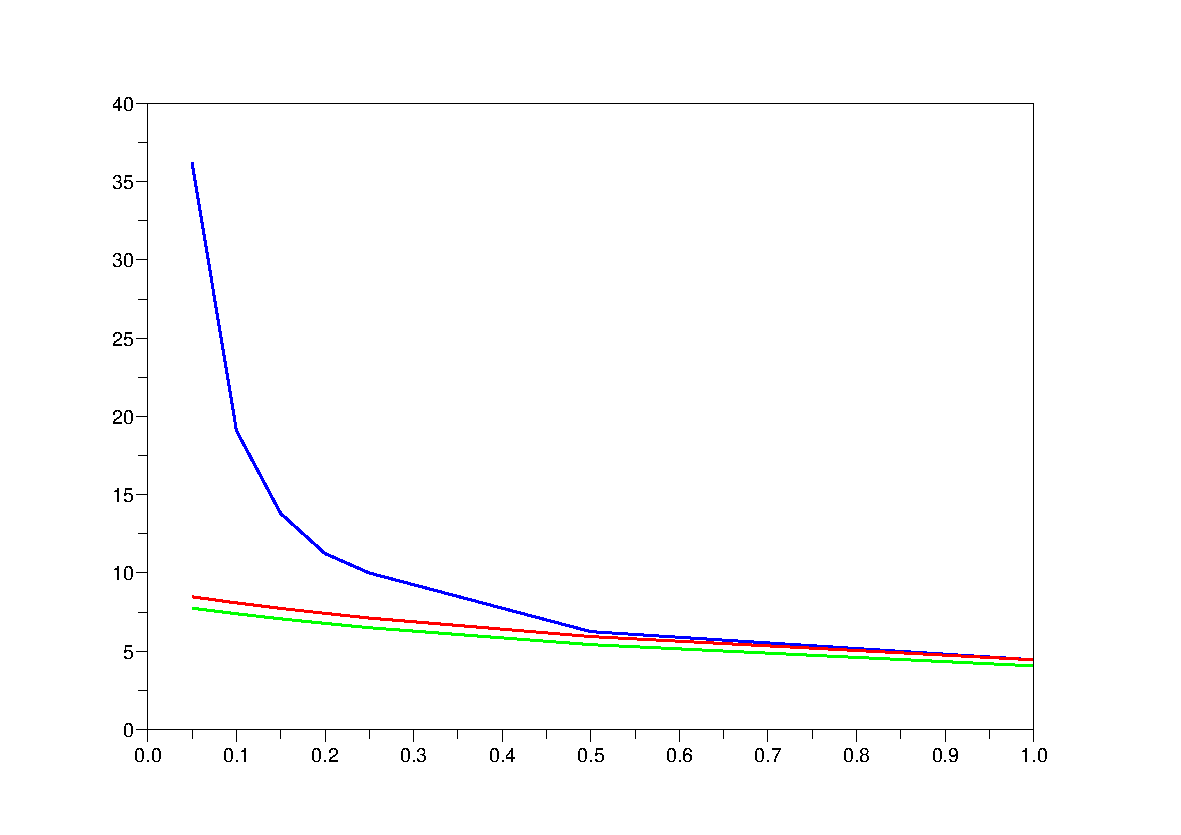
\includegraphics[width=0.6\columnwidth]{maxKcomparison}
% 		\caption{Maximum $k$ of proved stability versus D}
	\end{figure}

}

\frame{\frametitle{Conclusions}
	\begin{itemize}
		\item The problem of Absolute Stability has been introduced
		\item Classic solutions to the problem have been presented
		\begin{itemize}
			\item Circle Criterion
			\item Integral Quadratic Constraints
		\end{itemize}
		\item The concept of BIQC's has been introduced
		\item The adoption of a bias term in the IQC describing the nonlinear operator has allowed to reduce the conservativeness of these criteria
		\item A numerical example has also proved that BIQC's can be an effective tool to deal with uncertainties 
	\end{itemize}
}

% \section{A graphical criterion}

\frame{
  \frametitle{References}
% 	\bibliographystyle{plain}
	\bibliographystyle{../ijbc}
	\bibliography{../abstab}
}

\end{document}

